\chapter{Controlled Characterization of the Liquid State Machine}
\label{chap:lsm}

\section{Introduction and Purpose}
\label{sec:ch3_intro}

The first question the dissertation must answer is under what dynamical conditions the reservoir converts weak temporal structure in the input EEG into stable, discriminable state trajectories---that is, what operating regime makes hidden temporal order observable.

The theoretical foundations of reservoir computing, reviewed in Chapter~\ref{chap:background}, establish that a Liquid State Machine can, in principle, approximate any time-invariant causal operator with fading memory---provided that the separation and approximation properties are satisfied \cite{Maass2002RealTime, boyd_chua_1985}. However, universality is a statement about the existence of a sufficient reservoir, not a guarantee that any particular configuration will perform well on a specific signal class. The gap between the universality theorem and a functioning engineering system is filled by empirical characterization: systematic investigation of how the reservoir's controllable parameters---membrane time constant, firing threshold, network size, and feature extraction strategy---shape its driven response and determine the quality of the representations it produces.

The formal justification for treating the reservoir as an instrument for recovering hidden temporal order rests on the \emph{separation property} established by Maass, Natschl\"{a}ger, and Markram \cite{Maass2002RealTime}: if the reservoir satisfies the echo state condition, then different input histories produce distinguishable state trajectories. This is a mathematical guarantee that hidden temporal structure becomes observable in the reservoir's high-dimensional state space. The present chapter validates this condition empirically: the dominant Lyapunov exponent is $\lambda_1 = -0.054$ across $4{,}220$ measurements, confirming $100\%$ negative values and establishing that the reservoir operates in the contractive regime where the separation property holds. The experiments that follow identify the specific operating regime---the range of membrane time constants, thresholds, and temporal coding resolutions---in which this theoretical guarantee translates into practically useful discriminability for EEG-scale signals.

This chapter performs that characterization under controlled conditions. Its purpose is narrow and specific: to identify operating-regime parameters that produce stable, discriminative, spike-based reservoir responses to simple synthetic stimuli, and to understand \emph{why} those parameters produce those responses in terms of the underlying dynamical and information-processing principles. The resulting parameter selections are then carried forward as the provisional design specification for the embedding pipeline developed in Chapter~\ref{chap:embeddings} and the end-to-end SHAPE EEG evaluation in Chapter~\ref{chap:arspi_net}.

The methodological philosophy deserves explicit statement. Throughout this chapter, synthetic constant-amplitude pulses are used as controlled probes rather than as surrogates for clinical EEG. This is a deliberate and standard engineering practice: just as an electrical engineer characterizes an amplifier's gain, bandwidth, and linearity with standardized test signals before deploying it in a complex circuit, this chapter characterizes the reservoir's temporal integration, dynamic range, and readout geometry with simplified inputs before exposing it to the noisy, nonstationary, and inter-subject-variable signals of real EEG. Controlled inputs permit clean analysis of cause-and-effect relationships between parameter choices and reservoir behavior---relationships that would be confounded by the many simultaneous sources of variability in clinical data. All quantitative claims in this chapter are statements about reservoir characterization under simplified excitation. The transfer of these findings to real EEG is an empirical question addressed in Chapter~\ref{chap:arspi_net}.

The chapter is organized as four experimental modules, each building on the findings of its predecessor. Each module answers a specific question about how hidden temporal order becomes observable---or fails to become observable---under different reservoir operating conditions:
\begin{enumerate}
    \item \textbf{Module 1} (Section~\ref{sec:module1}): \emph{What temporal scale of hidden order does the reservoir preserve?} The membrane decay parameter $\beta$ controls the reservoir's temporal integration window. This module identifies the regime in which the reservoir's fading memory is matched to the timescale of the input's discriminative structure.
    \item \textbf{Module 2} (Section~\ref{sec:module2}): \emph{Which dynamical regime makes hidden structure most stably observable?} The transition from subthreshold to spiking response fundamentally changes the reservoir's state-space geometry. This module demonstrates that the spiking regime produces more stable, reproducible, and interpretable representations---a direct consequence of the threshold-and-reset contraction that regularizes the population code.
    \item \textbf{Module 3} (Section~\ref{sec:module3}): \emph{Where in the temporal response does the hidden order reside?} Windowed readout analysis localizes discriminative information to the early post-stimulus window, establishing the temporal region where the reservoir's state is maximally driven and most informative.
    \item \textbf{Module 4} (Section~\ref{sec:module4}): \emph{Has the reservoir's nonlinear transformation made hidden structure linearly accessible?} Comparative readout analysis tests whether the reservoir has achieved its intended representational purpose: projecting the input into a geometry where class boundaries are linearly separable---a prerequisite for both classification and interpretable downstream analysis.
\end{enumerate}

The reservoir architecture, neuron model, and discrete-time implementation are as described in Chapter~\ref{chap:background}, Sections~\ref{sec:neuron_models}--\ref{sec:discrete_lif}. The LIF dynamics follow Equation~\eqref{eq:lif_discrete} with the $\beta$--$\tau_m$ correspondence derived in Section~\ref{sec:discrete_lif}. Unless otherwise noted, the reservoir consists of 512 recurrently connected LIF neurons implemented via \texttt{snn.RLeaky} in the \texttt{snnTorch} library \cite{eshraghian_training_2023}, with fixed random input weights $\mathbf{W}^{\text{in}} \in \mathbb{R}^{512 \times 33}$ (Xavier uniform initialization) and fixed random recurrent weights $\mathbf{W}^{\text{rec}} \in \mathbb{R}^{512 \times 512}$.

\textbf{Reservoir size.} This chapter uses 512 neurons for all characterization experiments, providing a conservative upper bound on network capacity. Chapter~\ref{chap:embeddings} performs a reservoir-size ablation study and demonstrates that classification performance saturates at 256 neurons, which becomes the dissertation-wide specification. The characterization results reported here transfer directly to the 256-neuron configuration because the phenomena under study---temporal integration, threshold regularization, and temporal localization---are governed by single-neuron dynamics and population statistics rather than by network size.


%% ===================================================================
%% MODULE 1
%% ===================================================================
\section{Module 1: Impact of the Membrane Time Constant on Reservoir Dynamics}
\label{sec:module1}

\subsection{Theoretical Motivation}

The membrane time constant $\tau_m$ is the single most important parameter governing how an LIF reservoir processes temporal structure. To understand why, consider the reservoir from two complementary perspectives: the time-domain view of temporal integration and the frequency-domain view of spectral filtering.

In the time domain, the subthreshold impulse response of the LIF neuron is a truncated exponential $h(t) = (1/\tau_m)\,e^{-t/\tau_m}$ for $t \geq 0$, which Lindeberg proved is the uniquely determined time-causal smoothing kernel satisfying non-creation of new structures across temporal scales \cite{lindeberg_2016}. This is not a biological curiosity; it is a deep result from scale-space theory establishing that the exponential decay of the LIF membrane is the \emph{only} causal temporal smoothing operation that does not introduce spurious features into the signal. The membrane time constant $\tau_m$ controls the width of this smoothing kernel: larger $\tau_m$ integrates over wider temporal windows, effectively forming a longer ``memory'' of past input, while smaller $\tau_m$ restricts integration to a narrow window around the present.

In the frequency domain, the same kernel acts as a first-order low-pass filter with transfer function $H(f) = 1/(1 + j2\pi f \tau_m)$ and $-3$\,dB cutoff frequency $f_c = 1/(2\pi\tau_m)$. Each neuron therefore performs spectral filtering whose bandwidth is directly controlled by $\beta$: smaller $\beta$ (larger $\tau_m$) yields a narrower bandwidth that emphasizes slow fluctuations, while larger $\beta$ (smaller $\tau_m$) admits higher-frequency content at the cost of shorter memory. For a population of $N_{\text{res}}$ neurons sharing the same $\tau_m$, the entire reservoir applies the same spectral weighting to its input, which means the choice of $\beta$ determines which frequency components of the driving signal are preferentially retained in the reservoir state and which are attenuated.

This has a direct connection to the general theory of reservoir memory. Dambre et al.\ \cite{dambre_2012} proved a fundamental trade-off in reservoir computing: a reservoir cannot simultaneously maximize its linear memory capacity (how far into the past it can recall) and its nonlinear computational capacity (how complex a transformation it can perform on its input). Linear memory is maximized when the reservoir dynamics are strongly contracting ($\tau_m$ very large relative to the input timescale), while nonlinear computation benefits from dynamics closer to the edge of stability. The choice of $\tau_m$ therefore positions the reservoir along this trade-off curve: very large $\tau_m$ favors long-range memory at the expense of nonlinear richness, while small $\tau_m$ favors nonlinear transformation at the expense of memory depth.

For a reservoir intended to process EEG, the choice of $\tau_m$ has concrete engineering consequences. EEG signals contain frequency content spanning delta ($<4$\,Hz) through gamma ($>30$\,Hz) bands, and the transient responses of interest (such as event-related activity in post-stimulus epochs) evolve over timescales of tens to hundreds of milliseconds. The reservoir's intrinsic time constant must be compatible with these timescales: too fast, and the reservoir forgets relevant history before it can be read out; too slow, and distinct transient events are blurred together. This module quantifies this trade-off empirically by sweeping $\beta$ across an order of magnitude and measuring the resulting temporal persistence of the reservoir's driven response.

\subsection{Experimental Design}

The primary observable is the summed membrane potential across all reservoir neurons:
\begin{equation}
    V_{\text{summed}}[t] = \sum_{i=1}^{N_{\text{res}}} M_i[t]
    \label{eq:v_summed}
\end{equation}
which serves as a convenient aggregate state variable for comparing reservoir operating regimes. It is not claimed to be physiologically equivalent to a local field potential.

A standardized input pulse of amplitude 0.8 was applied to the first 5 of 33 input features, starting at time step 20 and lasting 10 steps, within a total simulation of 150 time steps. The $\beta$ parameter was varied across four values: $\beta \in \{0.01, 0.02, 0.05, 0.10\}$, corresponding to approximate time constants $\tau_m \approx \{100, 50, 20, 10\}$ simulation steps (see Section~\ref{sec:discrete_lif} for the exact $\beta$--$\tau_m$ relationship). For each condition, both $V_{\text{summed}}[t]$ traces and individual-neuron membrane potential heatmaps were recorded for qualitative and quantitative comparison.

\subsection{Results}

The variation of $\beta$ produced clear and systematic modulation of temporal persistence (Figure~\ref{fig:summed_beta_response}). At $\beta = 0.01$ ($\tau_m \approx 100$), the summed membrane potential rose during the input pulse (time steps 20--30) and remained highly elevated throughout the remainder of the 150 time-step simulation, demonstrating the reservoir's capacity for long-term memory of recent input. As $\beta$ increased, the duration of sustained activity decreased markedly. At $\beta = 0.02$ ($\tau_m \approx 50$), the decay was faster but still extended well beyond the stimulus offset. At $\beta = 0.05$ ($\tau_m \approx 20$), the activity returned closer to baseline within 20--30 steps post-stimulus. At $\beta = 0.10$ ($\tau_m \approx 10$), the response was tightly confined to the pulse duration, with rapid decay after pulse offset.

Individual-neuron heatmaps confirmed these global patterns at the single-unit level. Figure~\ref{fig:heatmap_beta_slow} ($\beta = 0.01$) shows widespread, prolonged depolarization persisting well beyond time step 100 across a large fraction of the 512 neurons. Figure~\ref{fig:heatmap_beta_fast} ($\beta = 0.05$) shows a much quicker return to baseline, with most neurons near resting potential within 30--40 steps of pulse offset. The correspondence between the single-neuron heatmaps and the global summed potential confirms that the observed temporal modulation is driven primarily by the intrinsic membrane dynamics of individual neurons---each independently leaking toward rest at a rate governed by $\beta$---rather than by emergent network-level effects such as recurrent re-excitation.

\begin{figure}[H]
    \centering
    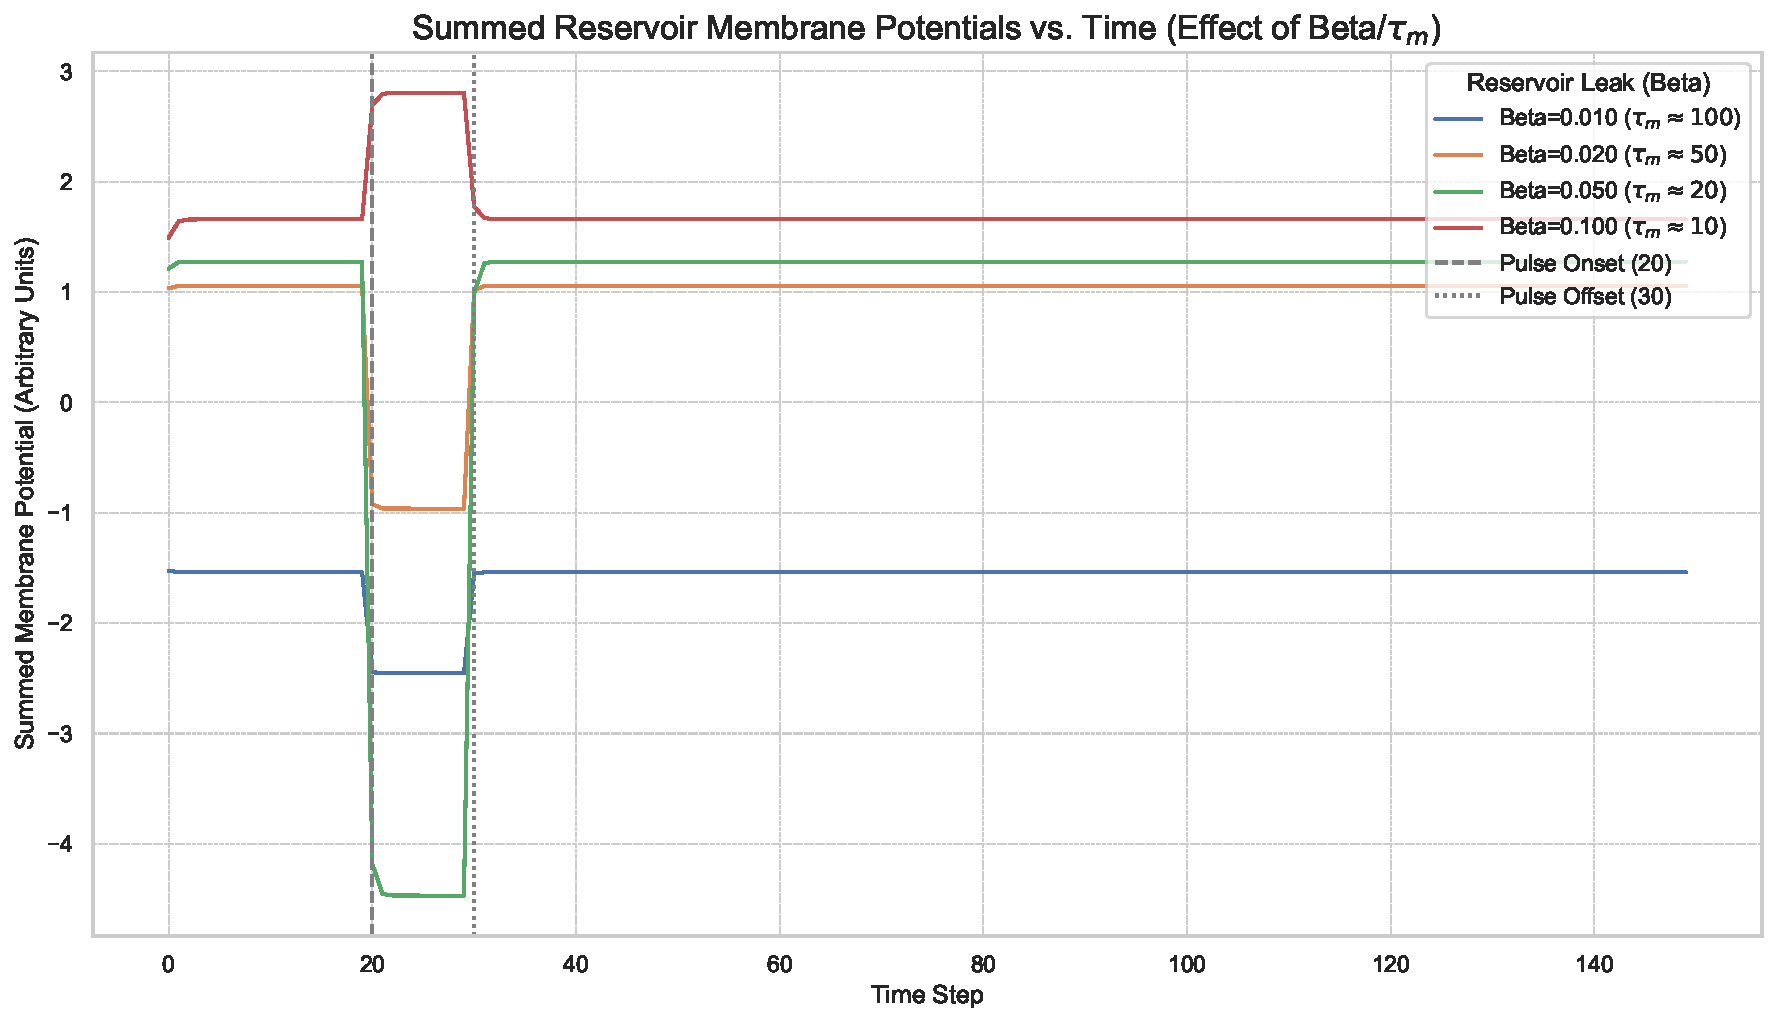
\includegraphics[width=0.9\textwidth]{pictures/chLSM/lsm_summed_activity_beta_comparison.pdf}
    \caption{Summed reservoir membrane potentials over time for different $\beta$ values. The input pulse was active from time step 20 to 30. Smaller $\beta$ (larger $\tau_m$) produces more sustained responses, consistent with first-order low-pass filtering.}
    \label{fig:summed_beta_response}
\end{figure}

\begin{figure}[H]
    \centering
    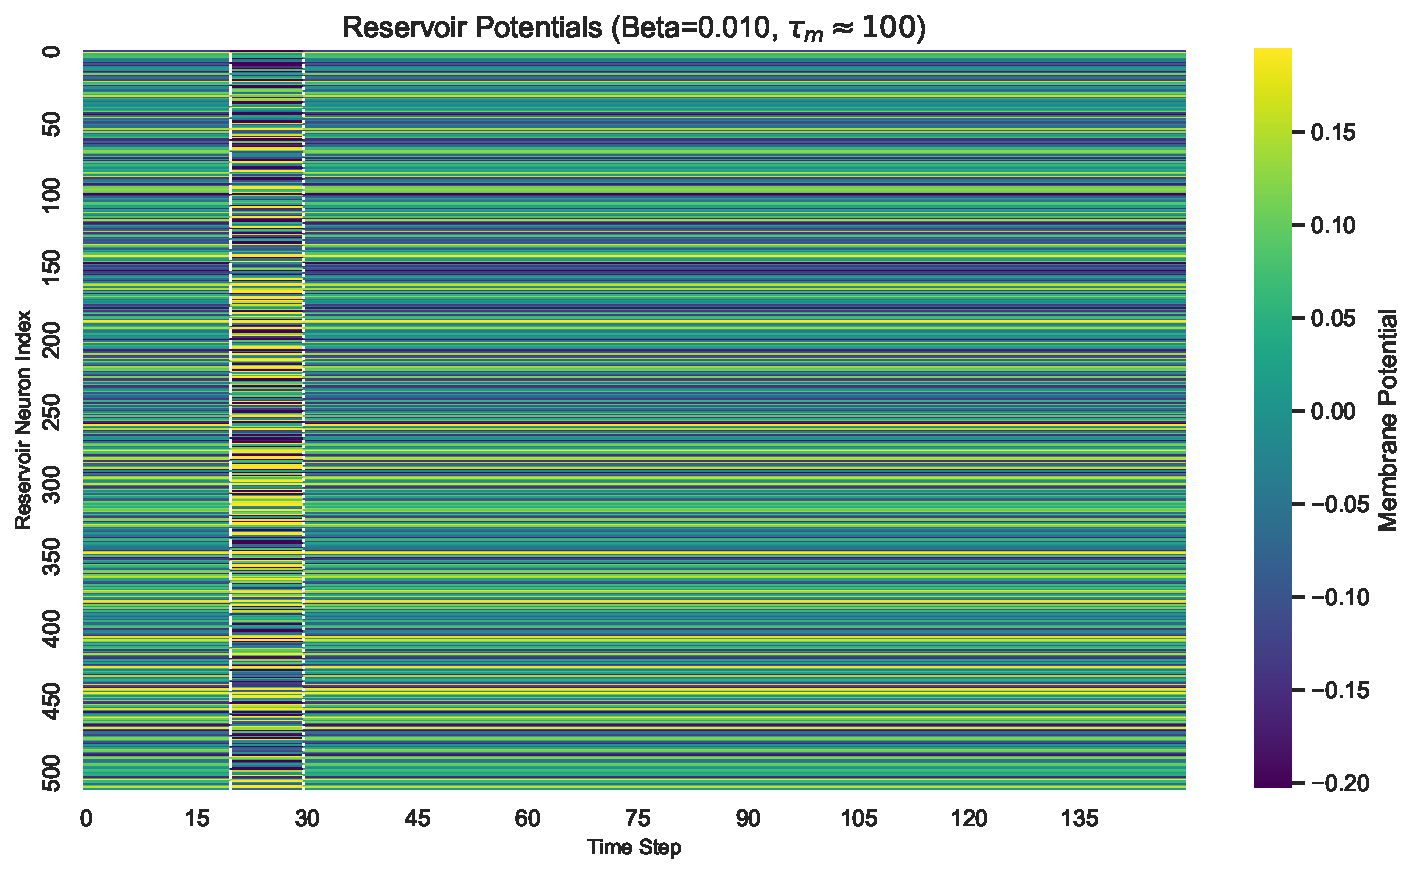
\includegraphics[width=0.8\textwidth]{pictures/chLSM/lsm_heatmap_beta_0p01.pdf}
    \caption{Heatmap of membrane potentials for all 512 reservoir neurons with $\beta = 0.010$ ($\tau_m \approx 100$). Activity is sustained across many neurons long after the input pulse, reflecting long temporal integration.}
    \label{fig:heatmap_beta_slow}
\end{figure}

\begin{figure}[H]
    \centering
    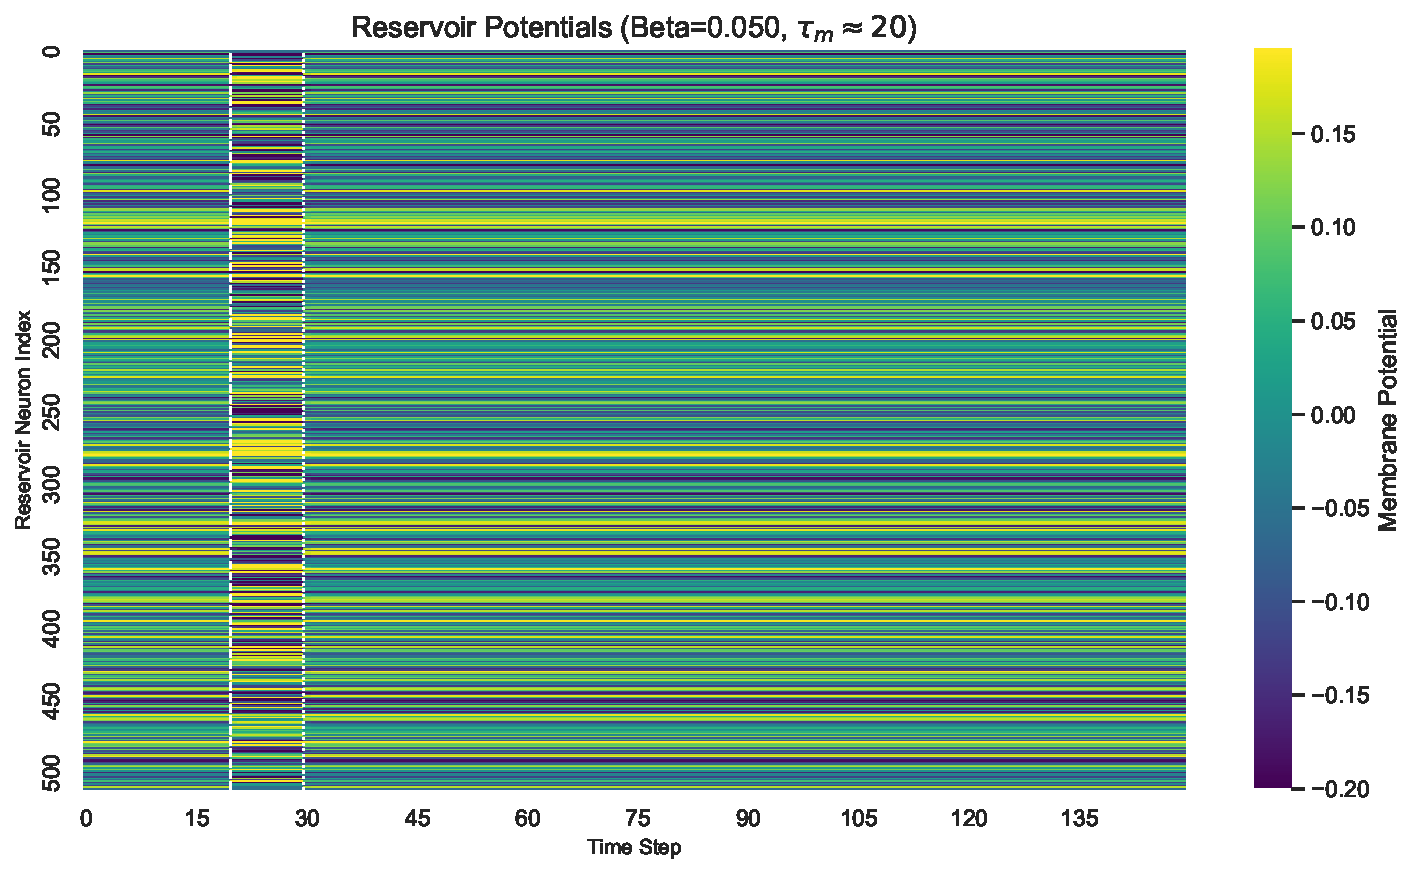
\includegraphics[width=0.8\textwidth]{pictures/chLSM/lsm_heatmap_beta_0p05.pdf}
    \caption{Heatmap of membrane potentials for all 512 reservoir neurons with $\beta = 0.050$ ($\tau_m \approx 20$). Activation is more transient, with most neurons returning to baseline within 30--40 steps of pulse offset.}
    \label{fig:heatmap_beta_fast}
\end{figure}

\subsection{Discussion and Significance}

These results validate the most fundamental requirement for reservoir-based temporal processing: that the reservoir's effective memory horizon can be systematically controlled through a single parameter. The relationship between $\beta$ and response persistence is well predicted by the LIF filter theory: the exponential decay kernel $h(t) = (1/\tau_m)\,e^{-t/\tau_m}$ implies that after $k$ time constants, only $e^{-k} \approx \{0.368, 0.135, 0.050, 0.018\}$ of the initial perturbation remains for $k \in \{1, 2, 3, 4\}$. The summed-potential traces in Figure~\ref{fig:summed_beta_response} are consistent with this prediction: the $\beta = 0.05$ trace ($\tau_m = 20$) has decayed substantially by step 60 ($k \approx 1.5$ after pulse offset), while the $\beta = 0.01$ trace ($\tau_m = 100$) retains most of its amplitude at step 150 ($k \approx 1.2$ after offset) \cite{gerstner_spiking_2002}.

The correspondence between the single-neuron heatmaps and the global summed potential confirms that the observed temporal modulation is driven primarily by the intrinsic membrane dynamics of individual neurons rather than by emergent network-level effects such as recurrent re-excitation. This is a useful diagnostic: it means that the temporal integration properties of the reservoir at this operating point are predictable from single-neuron theory, which simplifies the design process and makes the parameter choices more interpretable. In a strongly recurrent regime where network effects dominate, the relationship between $\beta$ and temporal persistence would be less transparent and harder to control.

From an information-theoretic perspective, the choice of $\tau_m$ determines the \emph{effective memory horizon} of the reservoir---the temporal depth over which the current state retains information about past inputs (Chapter~\ref{chap:background}, Section~\ref{sec:dynamical_systems}). This connects directly to the Dambre et al.\ \cite{dambre_2012} trade-off discussed in the theoretical motivation: a reservoir with very long memory ($\beta = 0.01$) retains more of the input history but applies a more nearly linear transformation (because the dynamics are strongly contracting), while a reservoir with short memory ($\beta = 0.10$) can perform more complex nonlinear transformations but loses longer-range dependencies. The choice $\beta = 0.05$ positions the reservoir at an intermediate point on this trade-off, and the empirical results confirm that it provides a practically useful balance: the response persists long enough to capture the immediate post-stimulus dynamics (the first 20--30 steps after the pulse) while decaying sufficiently to avoid blurring sequential events within a typical EEG epoch.

For the ARSPI-Net application specifically, the engineering requirement is that the reservoir's temporal footprint be compatible with the analysis windows used for feature extraction. The summed-potential traces confirm that $\beta = 0.05$ produces a response that is concentrated in a window of approximately 30--40 steps post-stimulus---a scale that is well matched to the Early Window (steps 20--50) tested in Module 3 and to the expanded feature window (steps 10--70) adopted in Chapter~\ref{chap:embeddings}. This alignment between the reservoir's intrinsic temporal scale and the feature extraction window is not coincidental; it reflects the fundamental principle that the feature representation should sample the reservoir state during the period of maximal input-driven activity, when the state carries the most information about the driving signal.


%% ===================================================================
%% MODULE 2
%% ===================================================================
\section{Module 2: Input Strength, Firing Threshold, and the Transition to Spiking}
\label{sec:module2}

\subsection{Theoretical Motivation}

Module 1 established control over the reservoir's temporal dynamics, but it did not address a more fundamental question: \emph{in which computational regime should the reservoir operate?} The LIF neuron has two qualitatively different operating modes, and the choice between them has profound consequences for the nature of the representations the reservoir produces.

Below the firing threshold $M_{\text{th}}$, the membrane potential evolves as a continuous analog variable governed by linear dynamics: $M_i[t] = (1 - \beta) M_i[t-1] + I_{\text{tot},i}[t]$. In this regime, the reservoir is a \emph{linear} dynamical system (since the LIF dynamics are linear below threshold) whose response to any input is a weighted superposition of the exponential modes determined by $\mathbf{W}^{\text{rec}}$. The specific superposition is set by the projection direction determined by $\mathbf{W}^{\text{in}}$. Different random $\mathbf{W}^{\text{in}}$ matrices excite different modes with different amplitudes, producing potentially very different global responses to the same input. This is a fundamental consequence of the linearity of the subthreshold dynamics: without any nonlinear mechanism to constrain the state-space trajectory, the full dimensionality of the random projection is preserved, and initialization-dependent differences can grow or persist indefinitely.

Above threshold, the neuron emits a spike and resets, introducing a strong piecewise nonlinearity that qualitatively changes the dynamics. The threshold-and-reset mechanism acts as a form of \emph{state-space contraction}: when $M_i[t] \geq M_{\text{th}}$, the membrane potential is reset to $M_{\text{reset}}$, erasing the precise pre-spike trajectory and replacing it with a stereotyped event. Regardless of the specific trajectory that brought the neuron to threshold---whether it arrived from a high or low initial potential, via a fast or slow approach---the post-reset state is the same. At the population level, this contraction has a regularizing effect: it reduces the sensitivity of the collective output to the specific $\mathbf{W}^{\text{in}}$ realization, because the threshold-crossing events produce the same reset regardless of the initialization-dependent trajectory that led to them.

This distinction between analog and digital operating regimes has a deep connection to the theoretical requirements for reservoir computing. The separation property of Maass et al.\ \cite{Maass2002RealTime} requires that different input signals be mapped to distinguishably different reservoir states. In the subthreshold regime, the states are distinguishable but highly dependent on the random projection; in the spiking regime, the states are distinguishable \emph{and} regularized by the threshold nonlinearity, making the representation more robust across instances. The approximation property, on the other hand, requires that the readout can extract the relevant information from the reservoir state. A state representation that is consistent across random initializations is far more useful for this purpose than one that requires instance-specific calibration.

This module empirically characterizes both regimes and tests which provides a more reliable basis for downstream feature extraction---a decision with direct architectural consequences for ARSPI-Net.

\subsection{Experimental Design}

Two threshold conditions were examined: $M_{\text{th}} = 1.0$ (high threshold, suppressing spiking) and $M_{\text{th}} = 0.5$ (low threshold, enabling spiking). For each condition, input pulse amplitudes of 0.6, 1.2, and 2.0 were applied (all other parameters as in Module~1, with $\beta = 0.05$). To assess initialization sensitivity in the subthreshold regime, the $M_{\text{th}} = 1.0$ condition was repeated across $N_{\text{instances}} = 5$ independent LSM instances, each with a newly initialized $\mathbf{W}^{\text{in}}$ (Xavier uniform) but identical $\mathbf{W}^{\text{rec}}$ and neuron parameters. The $M_{\text{th}} = 0.5$ condition was analyzed from a single representative instance, consistent with the exploratory objective of identifying a functional spiking regime.

Key observables included the summed membrane potential $V_{\text{summed}}[t]$ (Equation~\ref{eq:v_summed}), the instantaneous population firing rate $R[t] = (1/N_{\text{res}}) \sum_i S_i[t]$, the total spike count during the pulse window (steps 20--30), and the peak population firing rate.

\subsection{Results: Subthreshold Regime ($M_{\text{th}} = 1.0$)}
\label{sec:subthreshold_results}

In the subthreshold regime, the LSM's response was characterized by pronounced instance-to-instance variability. Different initializations of $\mathbf{W}^{\text{in}}$ produced qualitatively different response profiles: non-monotonic relationships between input amplitude and peak deflection (Figure~\ref{fig:instance1_thresh1_standalone}), consistent monotonic decreases (Figures~\ref{fig:instance2_thresh1_standalone},~\ref{fig:instance4_thresh1_standalone}), plateaus followed by sharp changes (Figure~\ref{fig:instance3_thresh1_standalone}), and nearly flat responses for some metrics (Figure~\ref{fig:instance5_thresh1_standalone}). When aggregated across all five instances (Figure~\ref{fig:summary_thresh1_new}), the average Peak Summed Potential (Min) showed a general downward trend with increasing input amplitude, but with standard deviations comparable to or exceeding the mean effect sizes. The Mean Summed Potential (Pulse) showed no clear aggregate trend.

This variability is not a bug in the implementation; it is a predictable consequence of the reservoir's geometry. Each $\mathbf{W}^{\text{in}}$ initialization creates a different linear projection of the 33-dimensional input into the 512-dimensional reservoir state space. Since the reservoir's recurrent dynamics are deterministic and fixed, the entire trajectory that follows is determined by this initial projection direction. In the subthreshold regime, without any nonlinear mechanism to regularize divergent trajectories, different projection directions lead to fundamentally different state-space orbits \cite{Norton2020_NextGenRC, Lukosevicius2009_Reservoir}. This means that the relationship between input amplitude and any aggregate observable (summed potential, peak deflection) is not a property of the reservoir architecture alone---it is jointly determined by the architecture and the specific random seed.

\begin{figure}[H]
    \centering
    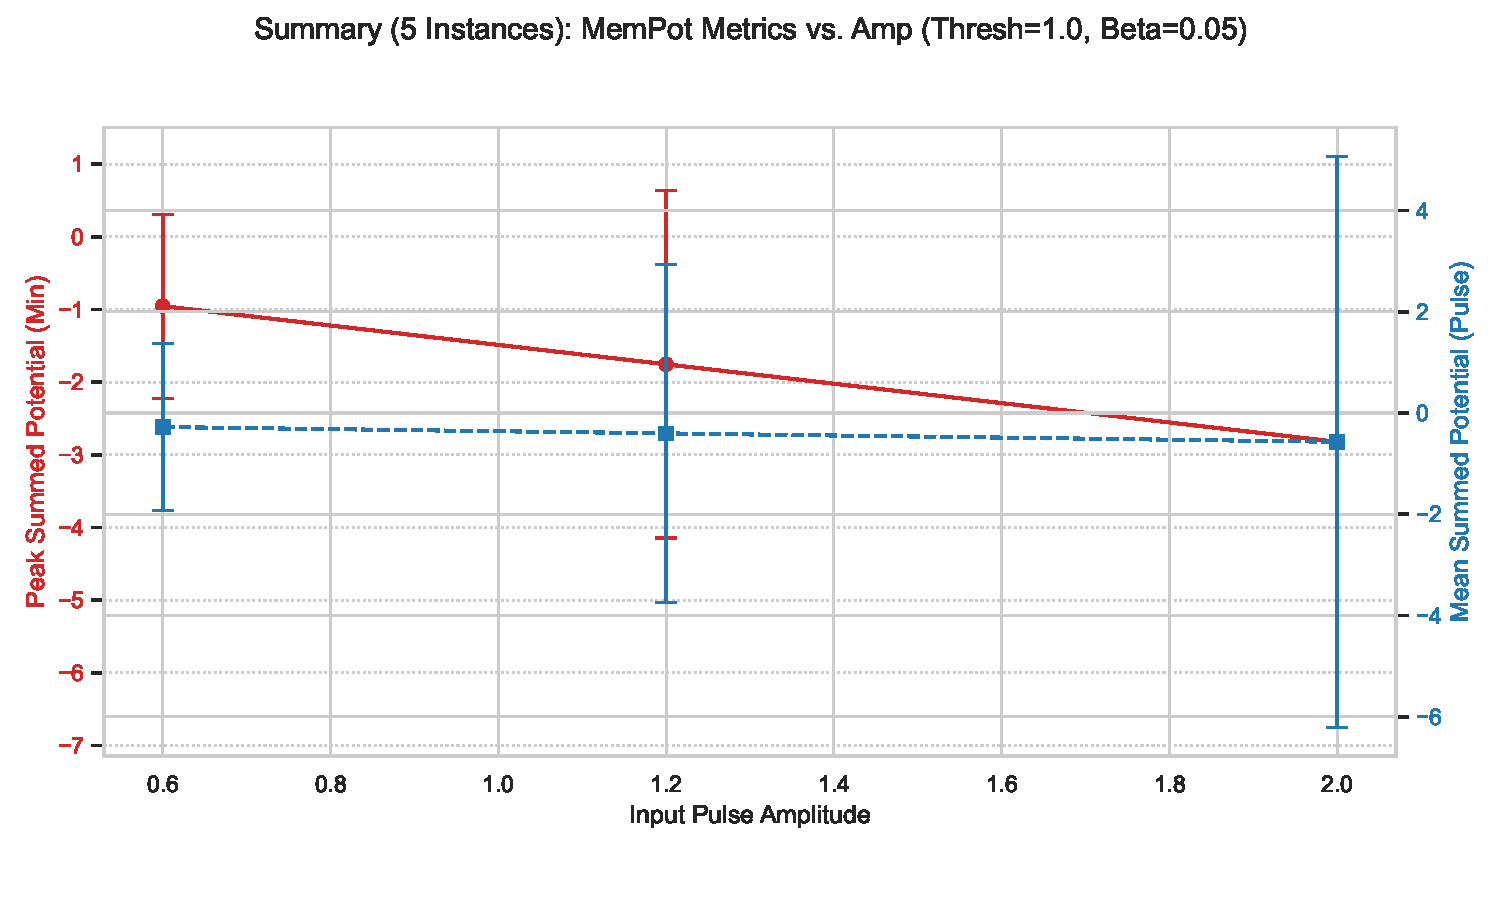
\includegraphics[width=0.7\textwidth]{pictures/chLSM/summary_mempot_metrics_thresh1p0.pdf}
    \caption{Summary of subthreshold metrics versus input amplitude across 5 network instances ($M_{\text{th}} = 1.0$, $\beta = 0.05$). Error bars represent standard deviation. The large variability reflects the sensitivity of continuous-valued trajectories to the random input projection.}
    \label{fig:summary_thresh1_new}
\end{figure}

\begin{figure}[H]
    \centering
    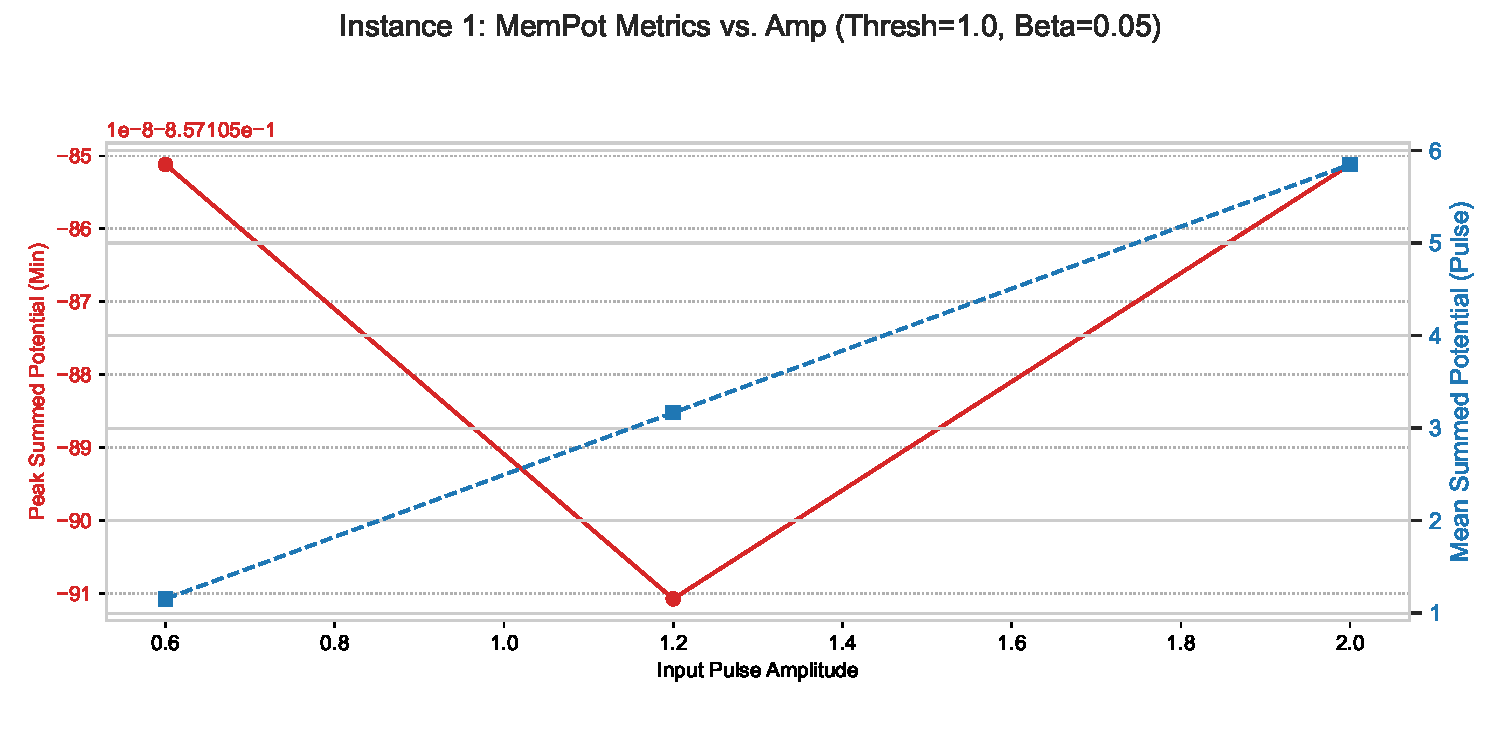
\includegraphics[width=0.7\textwidth]{pictures/chLSM/instance1_mempot_metrics_thresh1p0.pdf}
    \caption{Instance 1: Non-monotonic peak deflection, monotonically increasing mean potential.}
    \label{fig:instance1_thresh1_standalone}
\end{figure}

\begin{figure}[H]
    \centering
    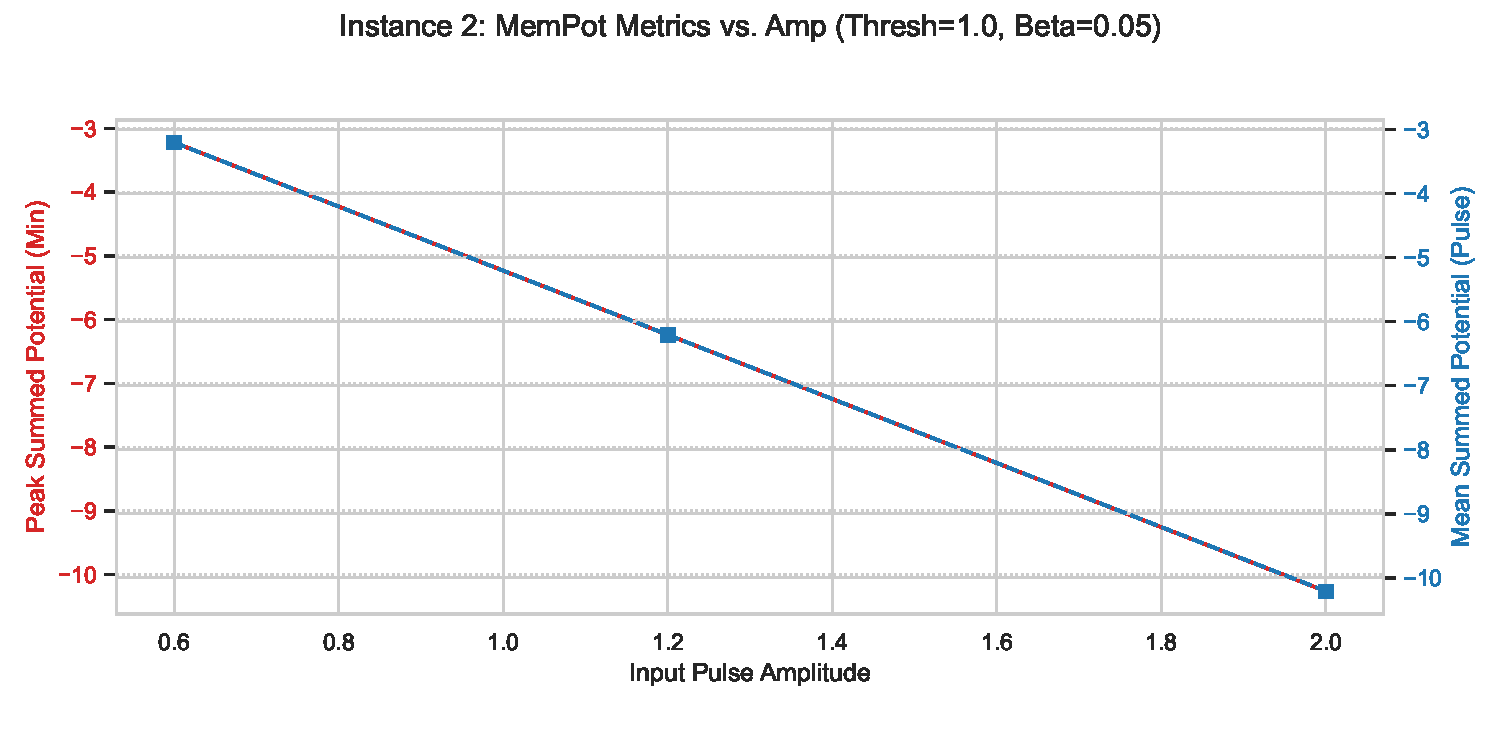
\includegraphics[width=0.7\textwidth]{pictures/chLSM/instance2_mempot_metrics_thresh1p0.pdf}
    \caption{Instance 2: Both metrics show strong monotonic decrease with input amplitude.}
    \label{fig:instance2_thresh1_standalone}
\end{figure}

\begin{figure}[H]
    \centering
    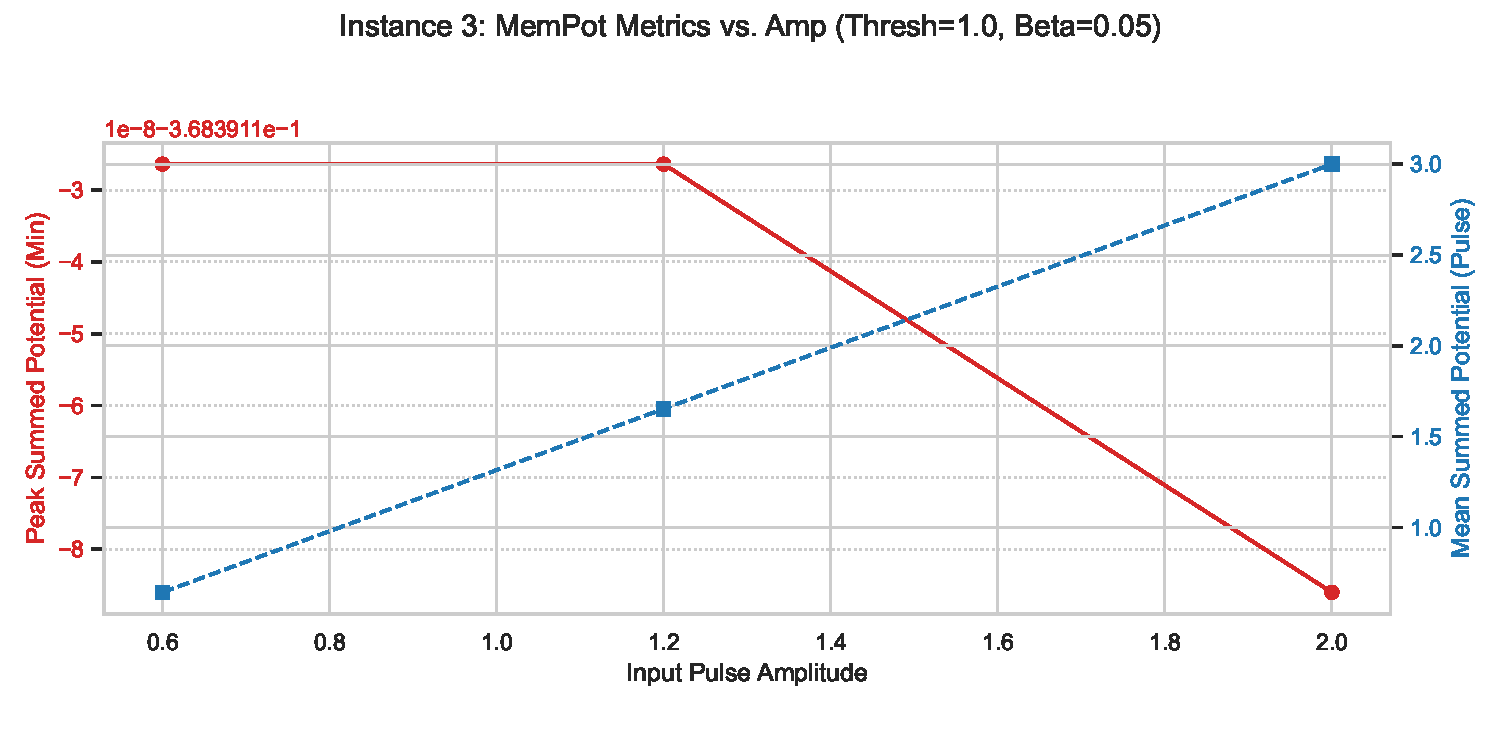
\includegraphics[width=0.7\textwidth]{pictures/chLSM/instance3_mempot_metrics_thresh1p0.pdf}
    \caption{Instance 3: Plateau followed by sharp decrease; monotonically increasing mean.}
    \label{fig:instance3_thresh1_standalone}
\end{figure}

\begin{figure}[H]
    \centering
    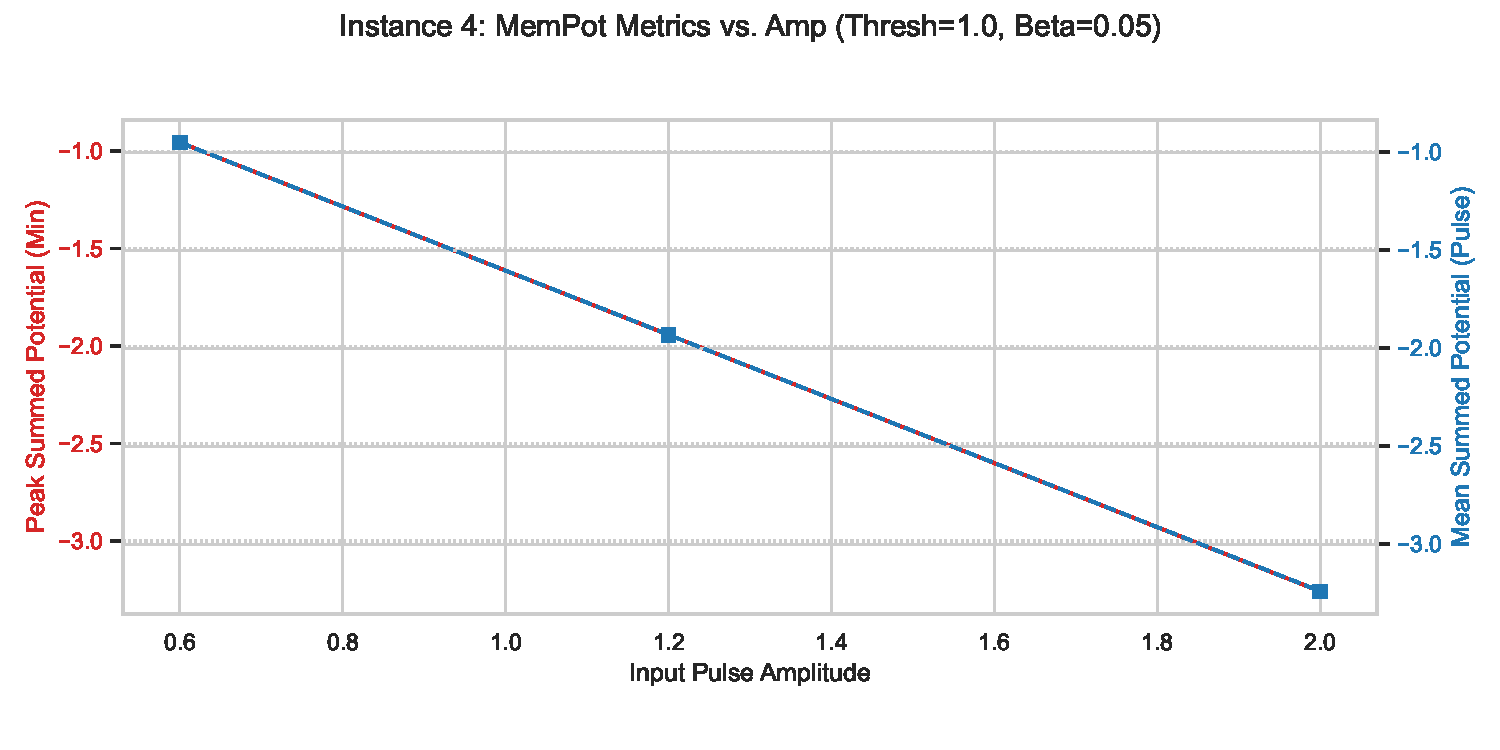
\includegraphics[width=0.7\textwidth]{pictures/chLSM/instance4_mempot_metrics_thresh1p0.pdf}
    \caption{Instance 4: Consistent monotonic decrease, similar to Instance 2.}
    \label{fig:instance4_thresh1_standalone}
\end{figure}

\begin{figure}[H]
    \centering
    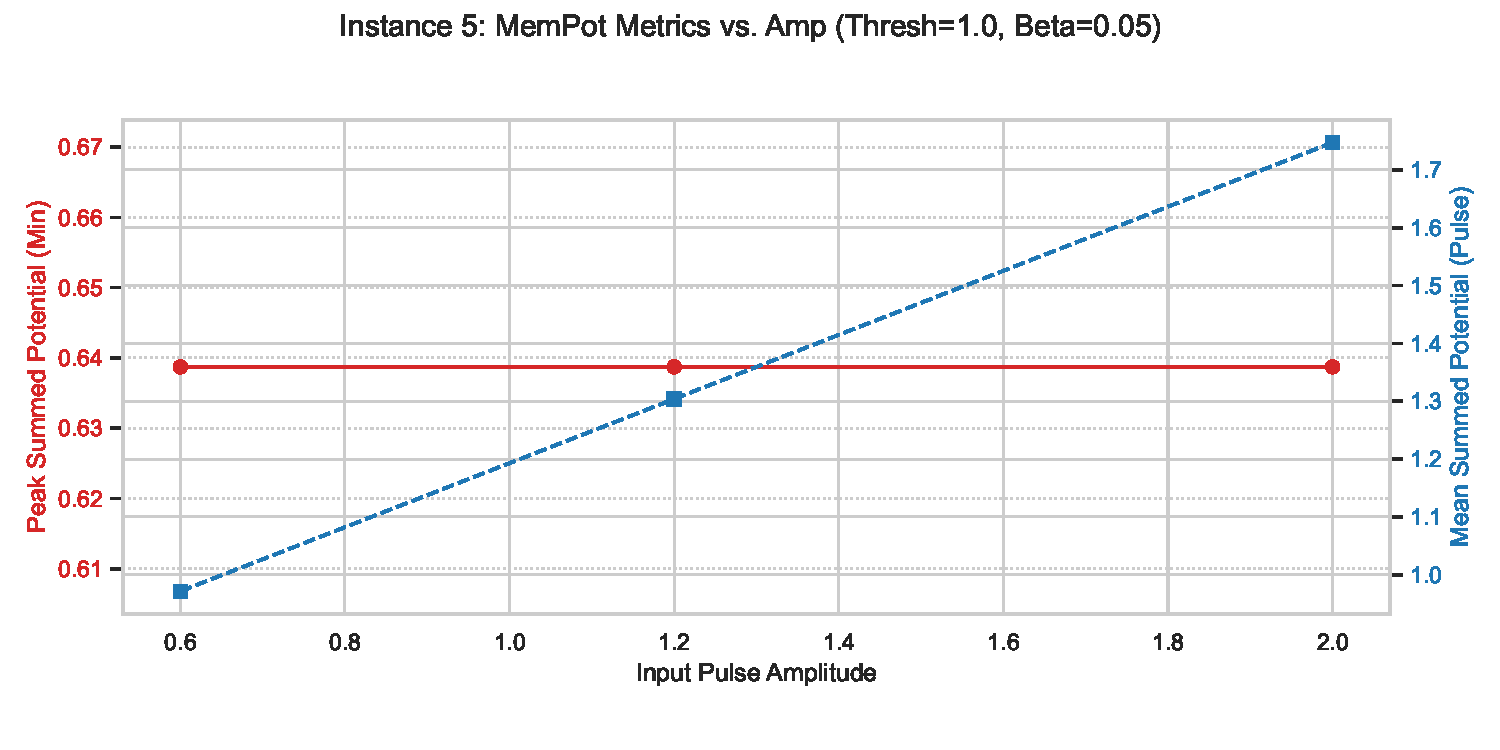
\includegraphics[width=0.7\textwidth]{pictures/chLSM/instance5_mempot_metrics_thresh1p0.pdf}
    \caption{Instance 5: Nearly constant peak deflection; monotonically increasing mean.}
    \label{fig:instance5_thresh1_standalone}
\end{figure}

\subsection{Results: Spiking Regime ($M_{\text{th}} = 0.5$)}
\label{sec:spiking_results}

Lowering the threshold to $M_{\text{th}} = 0.5$ fundamentally altered the reservoir's operational dynamics, enabling robust spiking activity that was clearly and systematically modulated by input strength.

The summed membrane potential (Figure~\ref{fig:m2_summed_mempot_thresh0p5_actual}) exhibited complex dynamics shaped by the interaction between input-driven depolarization and population spiking events. At low amplitude (0.6), which elicited minimal spiking, $V_{\text{summed}}[t]$ showed a modest positive deflection. At higher amplitudes (1.2 and 2.0), sharp negative deflections appeared, corresponding to synchronous firing and subsequent membrane reset events across many neurons simultaneously. The subthreshold metrics (Figure~\ref{fig:m2_mempot_metrics_thresh0p5_actual}) reflected this interaction: the Mean Summed Potential (Pulse) increased from amplitude 0.6 to 1.2 but sharply decreased for amplitude 2.0, because at higher amplitudes the negative-going population resets dominate the average.

The population firing rate (Figure~\ref{fig:m2_pop_firing_rate_thresh0p5_actual}) revealed the graded encoding of input strength with particular clarity. An amplitude of 0.6 elicited virtually no spikes---the input was insufficient to drive any significant fraction of neurons above the $M_{\text{th}} = 0.5$ threshold. Amplitude 1.2 produced a modest burst (peak rate $\sim$0.002 spikes/neuron/step, $\sim$5 total spikes during the pulse). Amplitude 2.0 produced a strong burst (peak rate $\sim$0.045 spikes/neuron/step, $\sim$170 total spikes). The quantitative relationship between input amplitude and spike output (Figure~\ref{fig:m2_spike_metrics_thresh0p5_actual}) shows a steep, nonlinear increase above the spike initiation threshold, with a clear transition between non-spiking and spiking behavior occurring between amplitudes 0.6 and 1.2.

\begin{figure}[H]
    \centering
    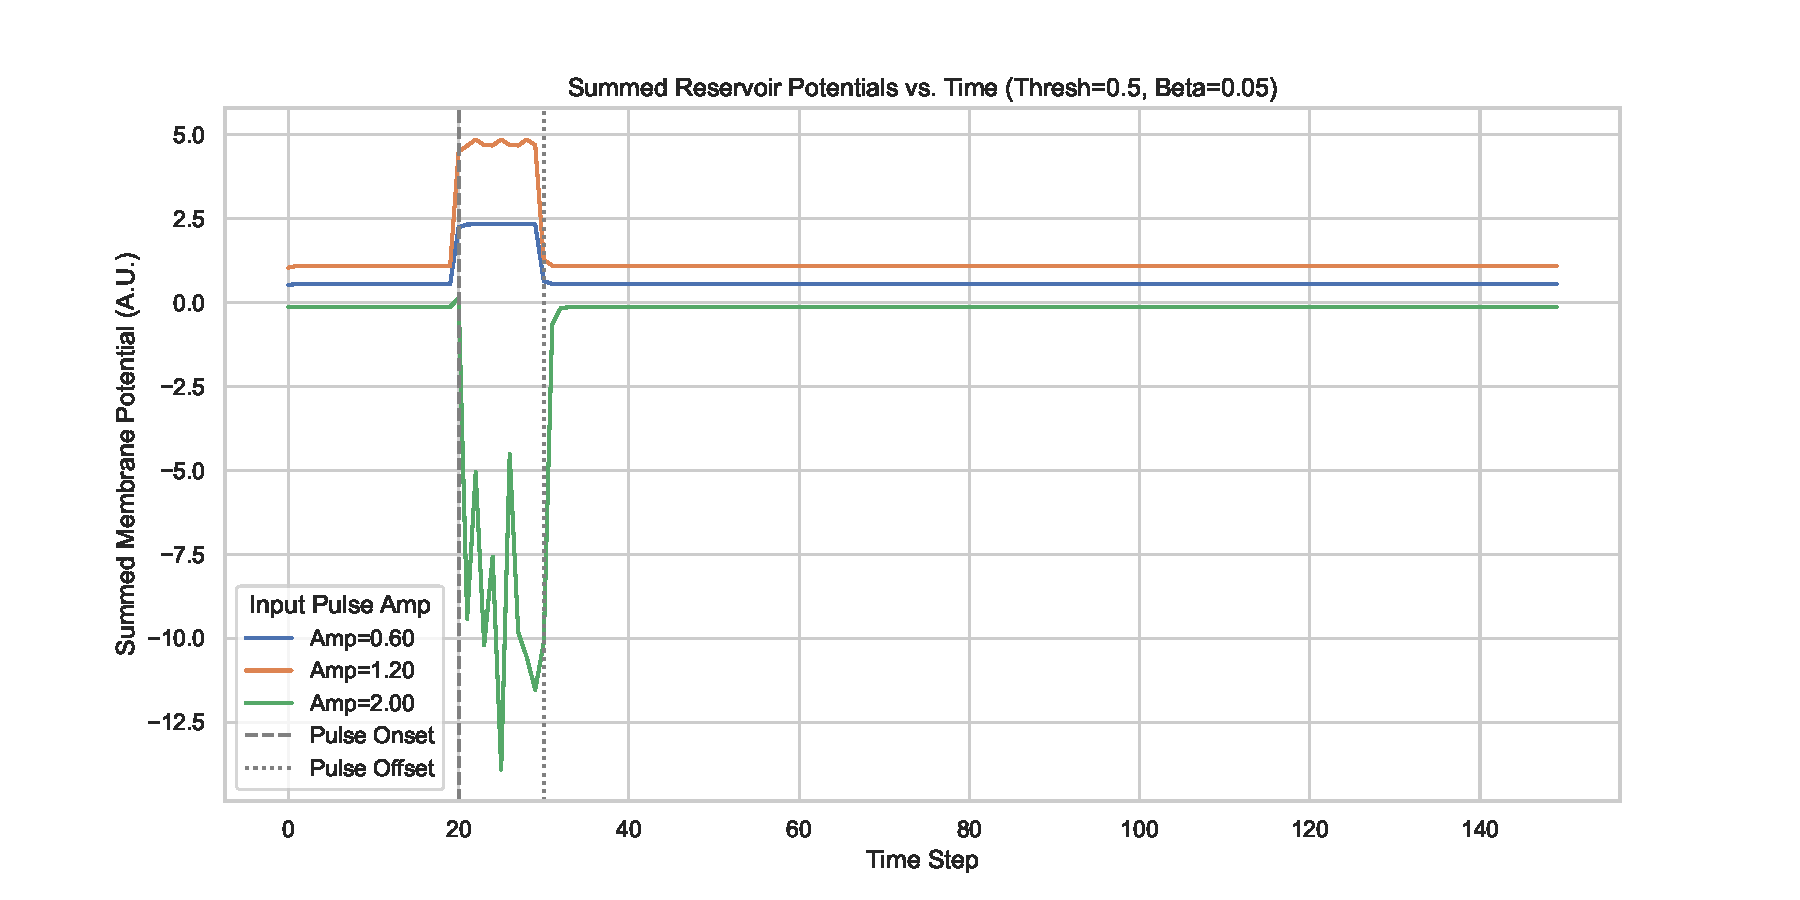
\includegraphics[width=0.9\textwidth]{pictures/chLSM/summed_mempot_thresh0p5.pdf}
    \caption{Summed membrane potentials in the spiking regime ($M_{\text{th}} = 0.5$, $\beta = 0.05$). Sharp negative deflections at higher amplitudes reflect synchronous spiking and membrane reset across the population.}
    \label{fig:m2_summed_mempot_thresh0p5_actual}
\end{figure}

\begin{figure}[H]
    \centering
    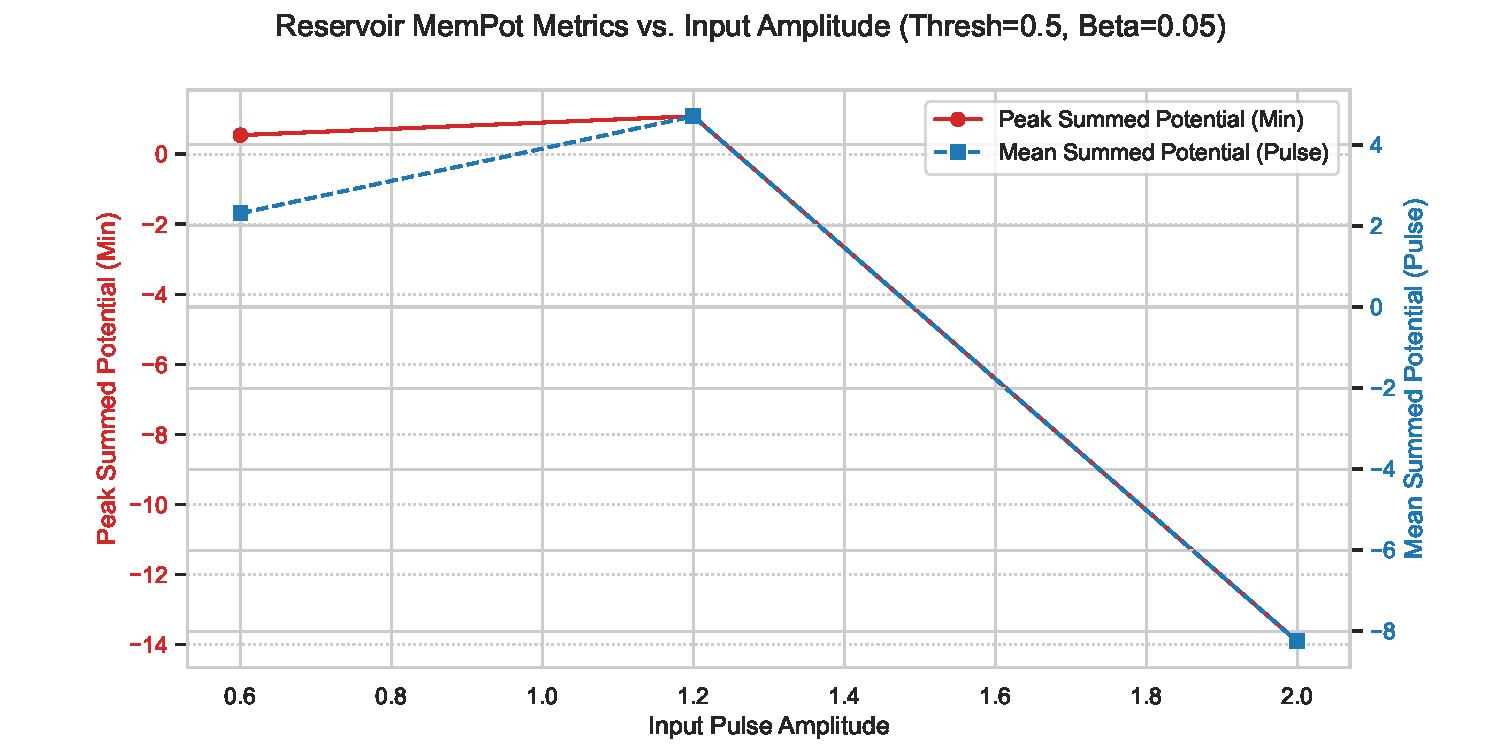
\includegraphics[width=0.8\textwidth]{pictures/chLSM/mempot_metrics_vs_amp_thresh0p5.pdf}
    \caption{Subthreshold metrics versus input amplitude in the spiking regime. Complex behavior arises from the interaction of input-driven depolarization and population-level reset events.}
    \label{fig:m2_mempot_metrics_thresh0p5_actual}
\end{figure}

\begin{figure}[H]
    \centering
    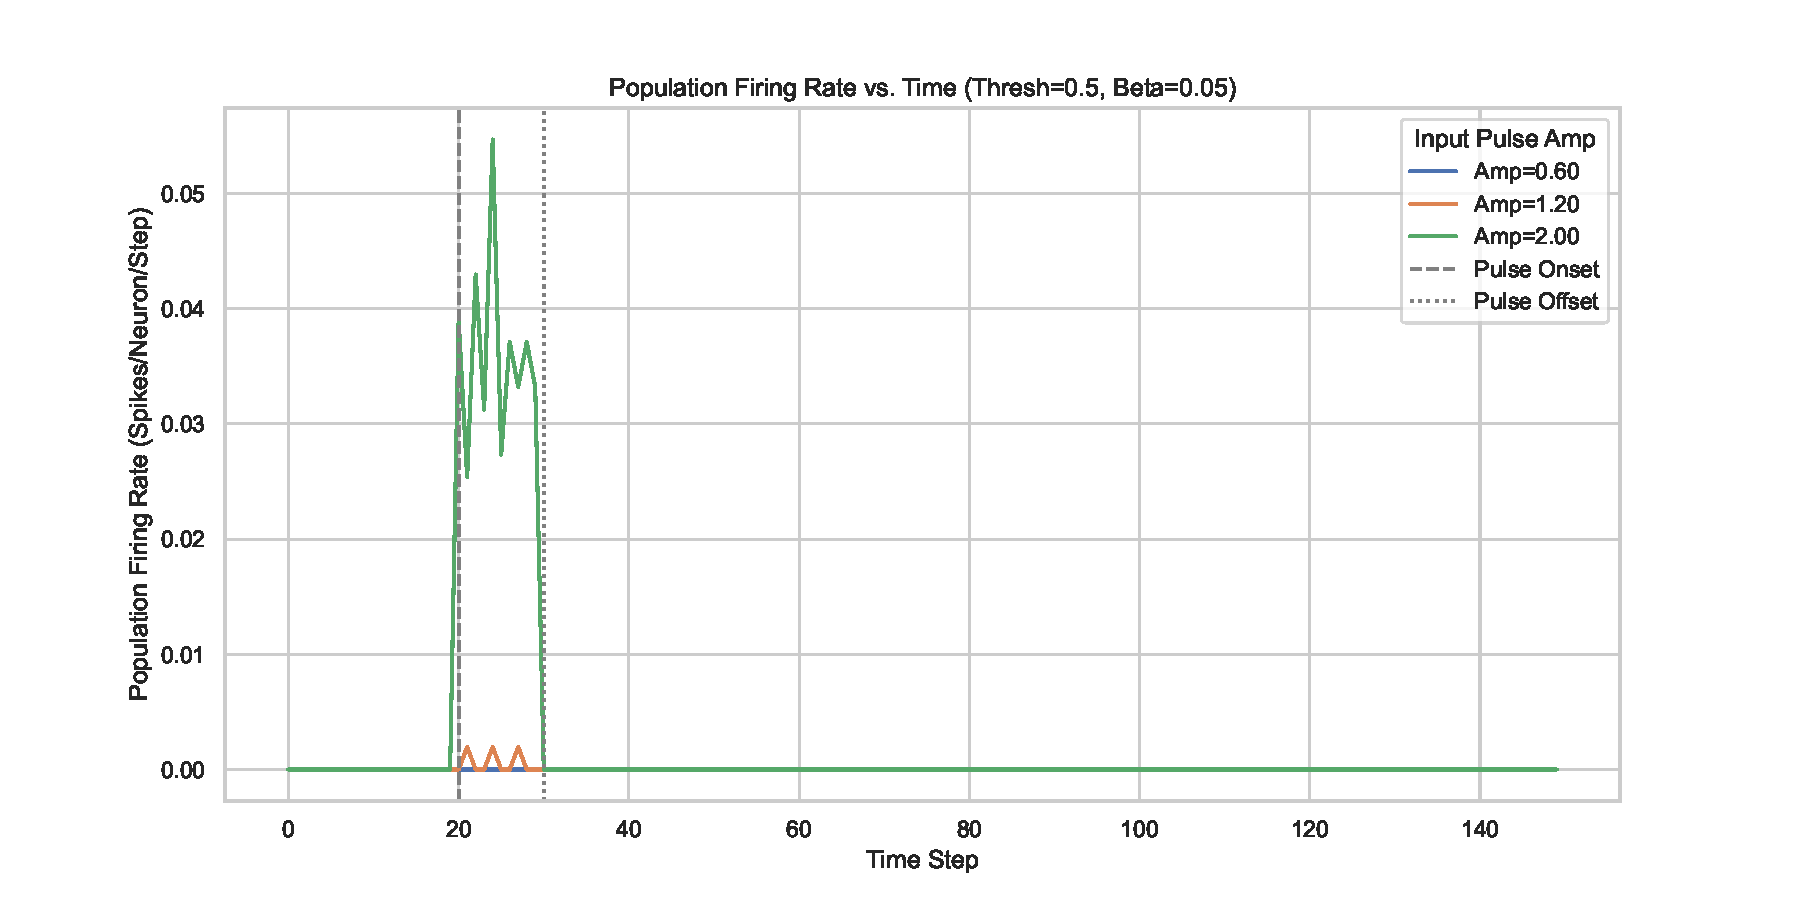
\includegraphics[width=0.9\textwidth]{pictures/chLSM/pop_firing_rate_thresh0p5.pdf}
    \caption{Population firing rate versus time for three input amplitudes ($M_{\text{th}} = 0.5$, $\beta = 0.05$). Spiking is clearly elicited and graded by input strength, demonstrating the reservoir's capacity for amplitude encoding in the spiking regime.}
    \label{fig:m2_pop_firing_rate_thresh0p5_actual}
\end{figure}

\begin{figure}[H]
    \centering
    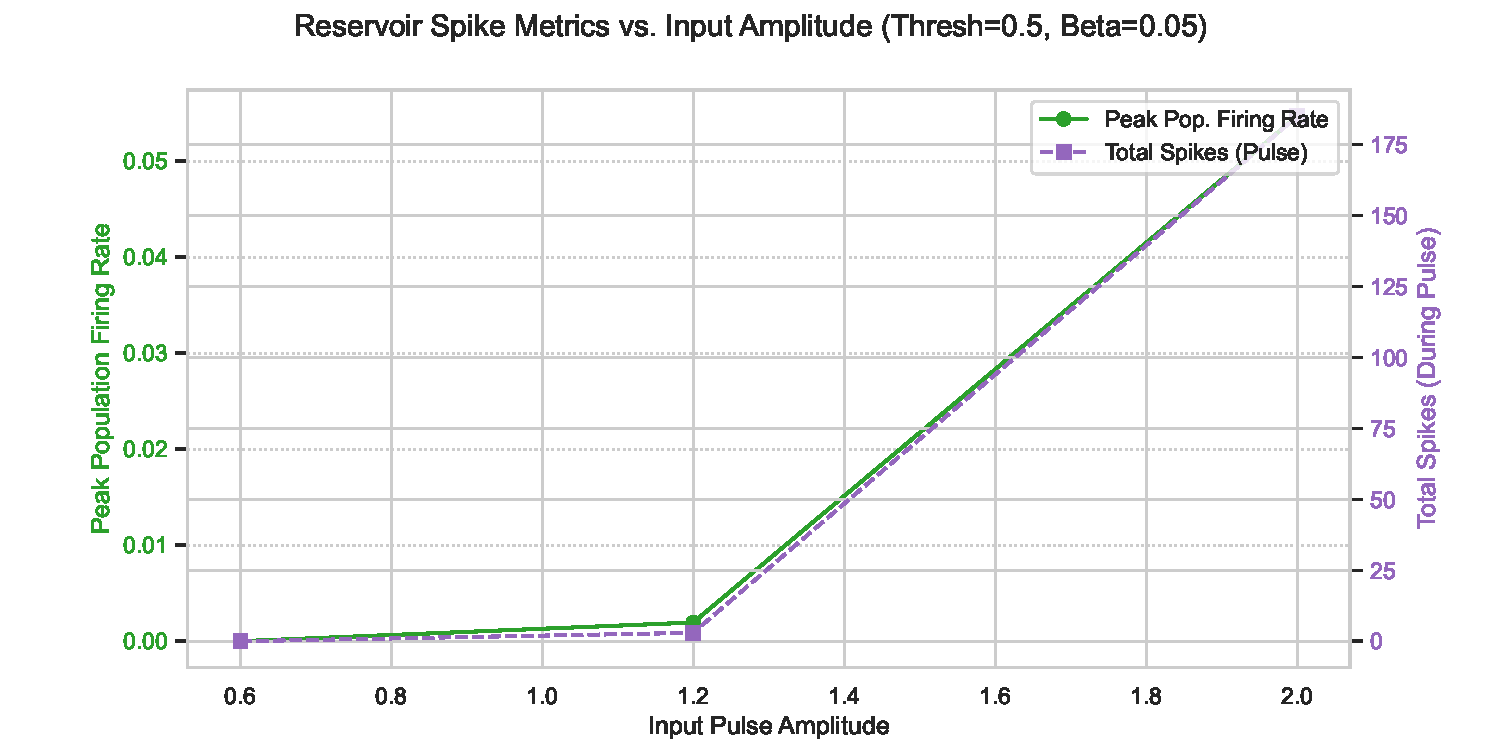
\includegraphics[width=0.8\textwidth]{pictures/chLSM/spike_metrics_vs_amp_thresh0p5.pdf}
    \caption{Peak population firing rate and total spike count versus input amplitude. Both metrics show a steep, nonlinear increase above the spike initiation threshold, consistent with the f-I curve of the LIF neuron scaled to the population level.}
    \label{fig:m2_spike_metrics_thresh0p5_actual}
\end{figure}

\subsection{Discussion and Significance}
\label{sec:module2_discussion}

The contrast between the subthreshold and spiking regimes is the central finding of this module, and its implications for ARSPI-Net architecture extend beyond mere parameter selection.

\subsubsection{The Regularizing Role of the Spiking Nonlinearity}

In the subthreshold regime, the reservoir operates as a high-dimensional linear dynamical system (since the LIF dynamics are linear below threshold). The response to any input is a weighted superposition of the exponential modes determined by $\mathbf{W}^{\text{rec}}$, and the specific superposition is set by the projection direction determined by $\mathbf{W}^{\text{in}}$. Different random $\mathbf{W}^{\text{in}}$ matrices excite different modes with different amplitudes, leading to the diverse and inconsistent response profiles documented in Figures~\ref{fig:instance1_thresh1_standalone}--\ref{fig:instance5_thresh1_standalone}. The implication is that subthreshold reservoir dynamics are \emph{not} a reliable basis for feature extraction when the specific network initialization is not controlled, because the input-output mapping is jointly determined by the architecture and the random seed.

The transition to the spiking regime introduces a qualitative change in the dynamics. The threshold-and-reset mechanism is a piecewise nonlinearity: when $M_i[t] \geq M_{\text{th}}$, a spike is emitted and the membrane potential is reset, erasing the precise pre-spike trajectory and replacing it with a stereotyped event. This mechanism acts as a form of state-space contraction: regardless of the specific trajectory that brought the neuron to threshold, the post-reset state is the same. At the population level, this contraction has a regularizing effect---it reduces the sensitivity of the collective output to the specific $\mathbf{W}^{\text{in}}$ realization and produces a population code that is more consistent across instances.

\subsubsection{The Population Rate Code and Its Engineering Significance}

The graded spiking response observed in Figures~\ref{fig:m2_pop_firing_rate_thresh0p5_actual}--\ref{fig:m2_spike_metrics_thresh0p5_actual} is a predictable consequence of the LIF neuron's frequency-current (f-I) relationship. Above the rheobase current, the firing frequency $f$ increases monotonically with input current $I$ following the relation $f = 1/(T_{\text{ref}} + \tau_m \ln[(R_m I - (V_{\text{reset}} - V_{\text{rest}}))/(R_m I - (M_{\text{th}} - V_{\text{rest}}))])$ \cite{gerstner_spiking_2002, dayan2001}. This f-I curve is a well-characterized property of the LIF model and provides a direct analytical link between the input amplitude and the single-neuron firing rate. At the population level, stronger inputs recruit more neurons above threshold and increase the firing rates of already-active neurons, producing a systematic, graded increase in both total spike count and peak firing rate. This graded population code is the basis for the feature extraction strategy used throughout the remainder of the dissertation.

The significance of this population rate code extends beyond simple amplitude encoding. In the context of reservoir computing, the population firing rate vector $\mathbf{r} = [r_1, r_2, \ldots, r_{N_{\text{res}}}]$ constitutes a high-dimensional representation of the input. Because different neurons have different input weights $\mathbf{W}^{\text{in}}_{i,:}$ and different recurrent connectivity patterns, they reach threshold at different input amplitudes and with different temporal profiles. The result is that the population rate vector is not simply a scaled version of the input; it is a nonlinearly transformed, high-dimensional expansion that preserves input information in a distributed format. This is precisely the representation that downstream classifiers and the graph model in Chapter~\ref{chap:arspi_net} will operate on.

The robustness of population-level spiking representations is further supported by theoretical work on coordinated spike coding. Boerlin, Machens, and Denève showed that spiking networks can achieve robust representations through collective error correction: neurons act coordinately to maintain the population readout within a bounded region of state space, making the representation resilient to perturbations including the kind of initialization-dependent variability documented in the subthreshold regime \cite{Boerlin2013_PredictiveCoding}. While the present reservoir is not explicitly designed for balanced coding, the empirical observation that its spiking output is systematically modulated by input strength across the tested dynamic range supports the practical viability of spike-based features for downstream inference.

\subsubsection{Implications for ARSPI-Net}

The architectural implication is direct: spike-based operation ($M_{\text{th}} = 0.5$) provides a more robust and reproducible basis for downstream feature extraction than purely subthreshold dynamics. The spiking regime yields a population code that is graded with respect to input strength, consistent across the tested conditions, and naturally suited to the binned spike-count and mean firing-rate features that form the basis of the embedding pipeline in Chapter~\ref{chap:embeddings}. The threshold setting $M_{\text{th}} = 0.5$ is therefore adopted alongside $\beta = 0.05$ as the second element of the provisional operating-point specification.


%% ===================================================================
%% MODULE 3
%% ===================================================================
\section{Module 3: Temporal Localization of Discriminative Information}
\label{sec:module3}

\subsection{Theoretical Motivation}

Modules 1 and 2 established the temporal and excitability parameters of the reservoir. The next critical question is \emph{where in time} the reservoir's response carries the information that a downstream readout can access. This question is distinct from the question of where the information \emph{exists} in the signal; it is specifically about where it is \emph{accessible via the chosen feature representation} (mean firing rates) given the reservoir's fading-memory dynamics.

The distinction between information existence and information accessibility is fundamental to the design of the feature extraction pipeline. The data processing inequality (Chapter~\ref{chap:background}, Section~\ref{sec:info_theory}) guarantees that the mutual information between the class label and the reservoir state cannot exceed the mutual information between the class label and the input. But even if the reservoir state at time $t$ retains some information about the input, that information may be encoded in subtle correlations among neuron states that a coarse feature representation (such as the population mean firing rate) cannot capture. The practical question for ARSPI-Net design is therefore not ``does the reservoir remember the input?'' but ``does the chosen feature representation preserve enough of what the reservoir remembers to support classification?''

The fading-memory property (Chapter~\ref{chap:background}, Section~\ref{sec:rc_theory}) provides the theoretical framework for answering this question. A reservoir with fading memory weights recent input history more strongly than remote history, with the weighting determined by the reservoir's contraction rate. For a reservoir with effective time constant $\tau_m \approx 20$ steps and a 10-step input pulse ending at step 30, this suggests that the most informative features should be concentrated in the temporal window immediately following the stimulus, with information content decaying approximately exponentially thereafter. However, the rate of information decay depends not only on $\tau_m$ but also on the recurrent dynamics: in principle, recurrent excitation could sustain stimulus-specific patterns beyond the single-neuron decay timescale by continuously re-exciting neurons whose activity would otherwise decay. This module tests empirically whether such sustained recurrent patterns exist in the current reservoir configuration or whether the information is indeed confined to the early post-stimulus window.

The answer has direct engineering consequences: it determines the optimal temporal window for feature extraction in the ARSPI-Net embedding pipeline and, more fundamentally, it tests whether the reservoir's memory capacity is sufficient to sustain class-specific information over the full analysis epoch or whether information is concentrated in a transient initial response.

\subsection{Experimental Design}

A binary classification task was defined: Class~0 (pulse amplitude 1.2) versus Class~1 (pulse amplitude 2.0), with 200 trials per class (400 total). For each trial, the reservoir's spike output from all 512 neurons was recorded over 150 time steps. Mean firing rates were extracted from four temporal windows:
\begin{itemize}
    \item \textbf{Early Window}: time steps 20--50 (stimulus onset plus 20 post-stimulus steps)
    \item \textbf{Late Window}: time steps 50--100
    \item \textbf{Full Response Window}: time steps 20--150
    \item \textbf{Entire Trial}: time steps 0--150
\end{itemize}
Each window produced a 512-dimensional feature vector per trial. Logistic regression with L2 regularization ($C = 0.1$) was trained separately on each window's features using 5-fold stratified cross-validation, with \texttt{StandardScaler} normalization fitted on each training fold and applied to the corresponding test fold.

\subsection{Results}

The results (Figure~\ref{fig:m3_accuracy_cv_comparison}) demonstrate a stark temporal dissociation. The Early Window, Full Response Window, and Entire Trial all achieved perfect mean accuracy ($1.000 \pm 0.000$) with zero standard deviation across folds. The Late Window performed at exact chance level ($0.500 \pm 0.000$).

The aggregated confusion matrices (Figure~\ref{fig:m3_confusion_matrices_cv}) provide further detail. For the Early Window (Figure~\ref{fig:m3_cm_cv_early}), all 200 Class~0 trials and all 200 Class~1 trials were correctly identified across the folds. For the Late Window (Figure~\ref{fig:m3_cm_cv_late}), all 400 test trials were predicted as Class~0---the classifier found no distinguishing structure in the late-window mean firing rates, producing a uniform prediction that maps every trial to the same class. The Full Response and Entire Trial windows (Figures~\ref{fig:m3_cm_cv_full},~\ref{fig:m3_cm_cv_entire}) showed perfect classification, driven by the inclusion of the informative early period.

\begin{figure}[H]
    \centering
    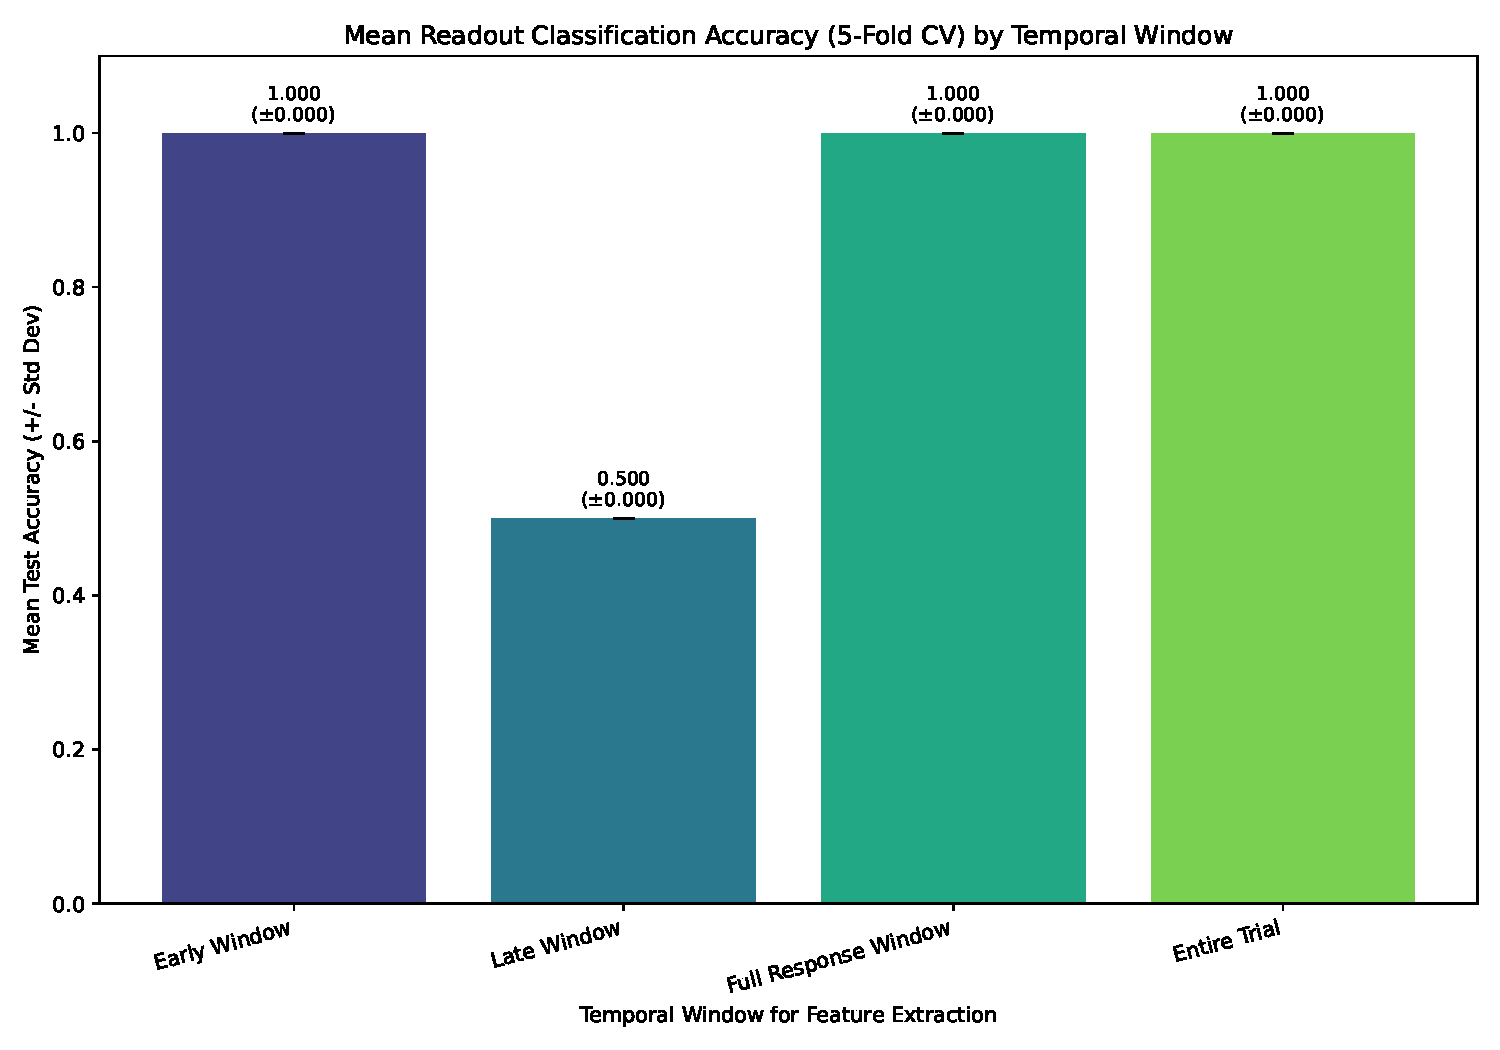
\includegraphics[width=0.9\textwidth]{pictures/chLSM/readout_accuracy_cv_comparison.pdf}
    \caption{Mean test accuracy (5-fold CV) for readouts trained on mean firing rates from different temporal windows. Discriminative information accessible via mean rates is concentrated in the Early Window. $\beta = 0.05$, $M_{\text{th}} = 0.5$.}
    \label{fig:m3_accuracy_cv_comparison}
\end{figure}

\begin{figure}[H]
    \centering
    \begin{subfigure}{0.48\textwidth}
        \centering
        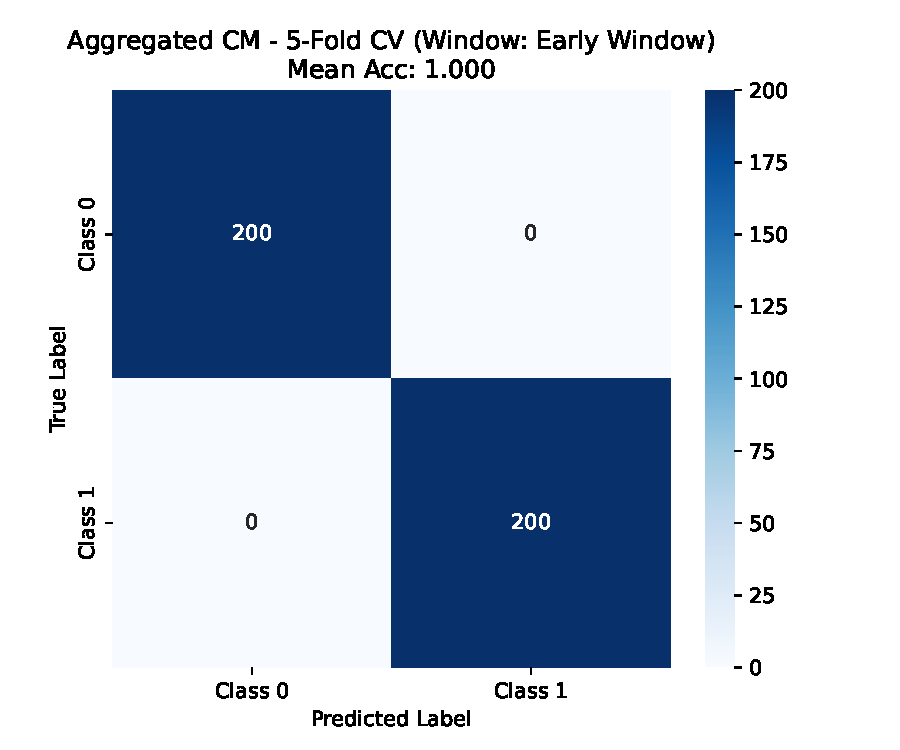
\includegraphics[width=\linewidth]{pictures/chLSM/confusion_matrix_cv_window_early_window.pdf}
        \caption{Early Window (Acc: 1.000)}
        \label{fig:m3_cm_cv_early}
    \end{subfigure}
    \hfill
    \begin{subfigure}{0.48\textwidth}
        \centering
        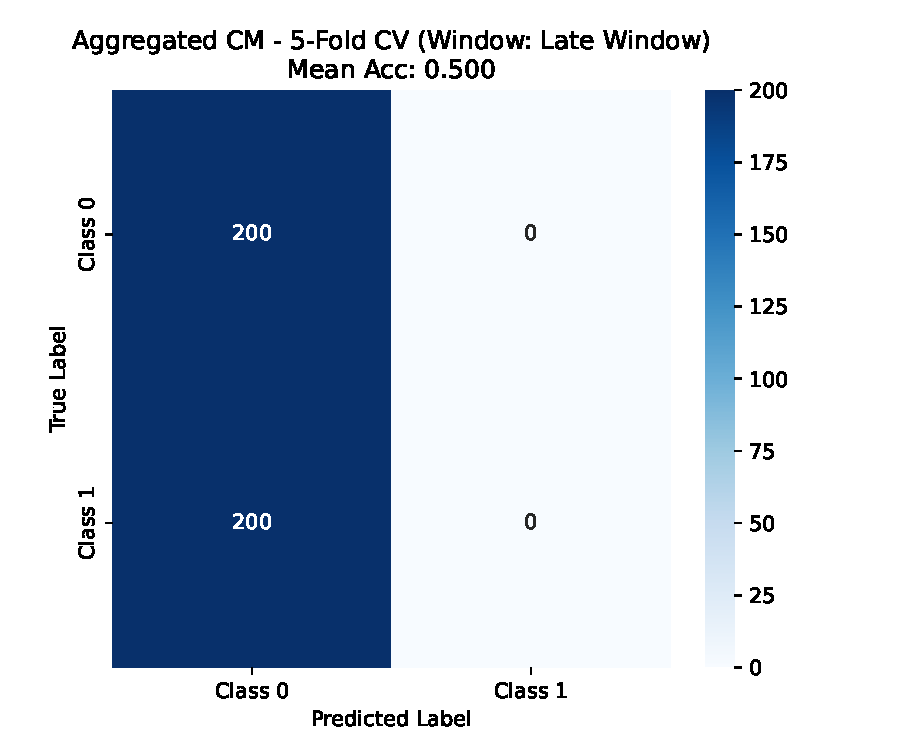
\includegraphics[width=\linewidth]{pictures/chLSM/confusion_matrix_cv_window_late_window.pdf}
        \caption{Late Window (Acc: 0.500)}
        \label{fig:m3_cm_cv_late}
    \end{subfigure}
    \vspace{1em}
    \begin{subfigure}{0.48\textwidth}
        \centering
        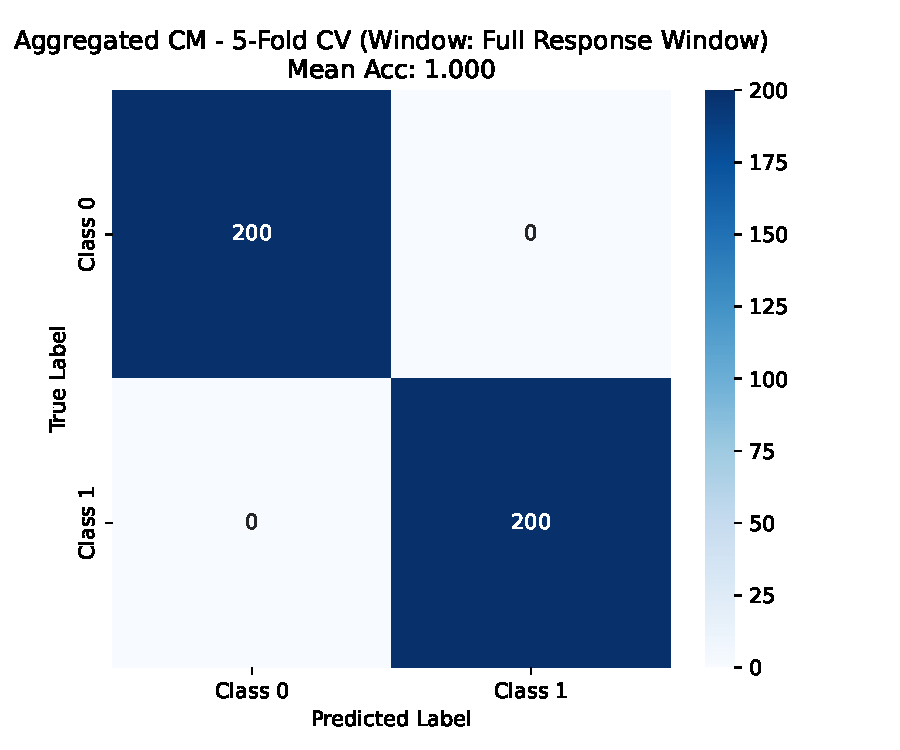
\includegraphics[width=\linewidth]{pictures/chLSM/confusion_matrix_cv_window_full_response_window.pdf}
        \caption{Full Response Window (Acc: 1.000)}
        \label{fig:m3_cm_cv_full}
    \end{subfigure}
    \hfill
    \begin{subfigure}{0.48\textwidth}
        \centering
        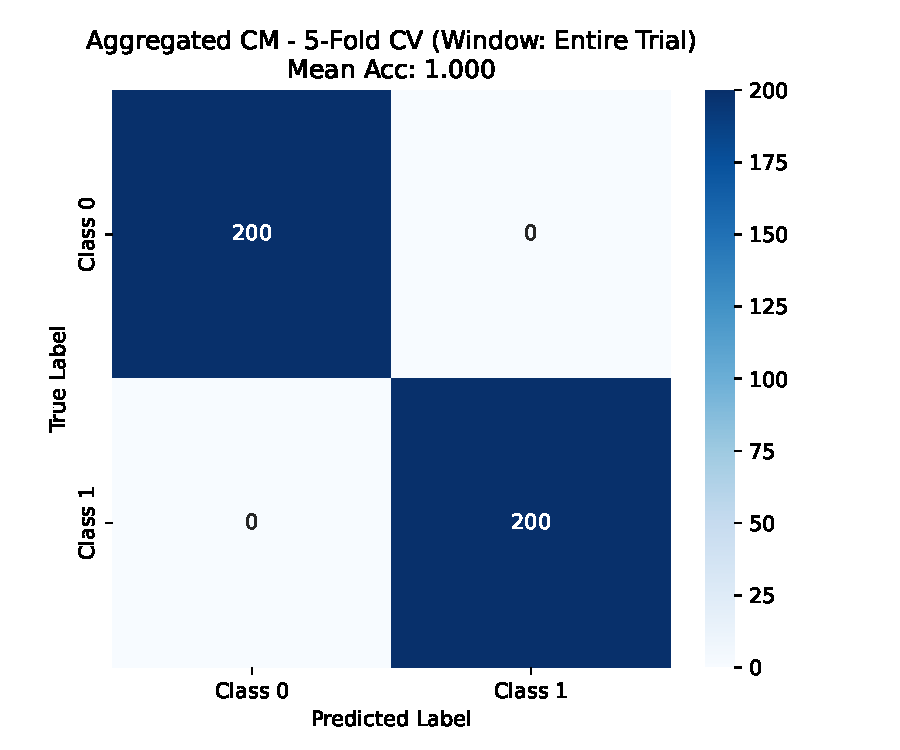
\includegraphics[width=\linewidth]{pictures/chLSM/confusion_matrix_cv_window_entire_trial.pdf}
        \caption{Entire Trial (Acc: 1.000)}
        \label{fig:m3_cm_cv_entire}
    \end{subfigure}
    \caption{Aggregated confusion matrices (5-fold CV) for each temporal window. $\beta = 0.05$, $M_{\text{th}} = 0.5$.}
    \label{fig:m3_confusion_matrices_cv}
\end{figure}

\subsection{Discussion and Significance}

\subsubsection{The Biophysical Basis of Information Decay}

The chance-level performance of the Late Window is a predictable and quantitatively accountable consequence of the LIF fading-memory dynamics. With $\beta = 0.05$ ($\tau_m \approx 20$ steps), any input-driven perturbation $\Delta M_0$ decays as $\Delta M(t') \approx \Delta M_0\, e^{-t'/\tau_m}$, where $t'$ is the time elapsed since input offset (step 30). The Late Window begins at step 50 ($t' = 20 = 1\tau_m$), where only $\sim$36.8\% of the initial perturbation remains, and extends to step 100 ($t' = 70 = 3.5\tau_m$), where only $\sim$3\% persists. The direct electrophysiological signature of the input stimulus is therefore substantially attenuated throughout this window.

This decay is compounded by the recurrent dynamics. After the external drive ceases and its immediate effects decay, the reservoir's activity is increasingly shaped by its autonomous dynamics---the intrinsic modes determined by $\mathbf{W}^{\text{rec}}$. These modes do not encode stimulus-specific information; they reflect the network's settled, input-agnostic behavior. The reservoir's state trajectories for the two stimulus classes, which were initially well-separated during the driven response, converge toward a common attractor as the input influence fades \cite{Sussillo2009, Barak2017}. The mean firing rate, which averages over the entire 50-step Late Window, is too coarse a feature to resolve any residual stimulus-specific structure that may persist in the fine-grained timing of individual spikes.

\subsubsection{What Information Decay Does and Does Not Imply}

Two scope considerations qualify this finding, and both have direct consequences for the embedding pipeline developed in the next chapter.

First, the chance-level result does \emph{not} imply that no information persists in later time steps---it implies only that the mean firing rate representation over 50-step averages cannot recover it. The mean firing rate is a maximally coarse temporal feature: it collapses all temporal structure within the window into a single scalar per neuron. If stimulus-specific information persists in the form of precise spike timing differences, evolving patterns of synchrony among neuron subpopulations, or the activity of sparse but consistently firing ensembles, the mean rate would be blind to all of these. More temporally resolved features, such as the binned spike counts developed in Chapter~\ref{chap:embeddings}, partition the window into shorter bins that may capture residual temporal structure invisible to the coarse mean-rate feature. This observation directly motivates the BSC$_6$ coding scheme validated in the next chapter, which replaces the single mean rate with six temporally resolved bins per neuron.

Second, the homogeneity of neuronal time constants in the current reservoir (all neurons share the same $\beta = 0.05$) may contribute to a more uniform and rapid loss of stimulus-specific information than would occur in a heterogeneous network. When all neurons decay at the same rate, the population-level memory of a transient input decays at that same rate, because there are no slow neurons to maintain a persistent trace. Theoretical and empirical work suggests that neuronal heterogeneity---a diversity of intrinsic timescales within the same network---can significantly enrich the dynamical repertoire of recurrent networks and expand their capacity to maintain and encode input features over longer durations \cite{Kim2024NeuralHeterogeneity}. A reservoir with a distribution of $\beta$ values would contain some slow-leaking neurons ($\beta \approx 0.01$) that retain input traces long after the fast neurons have returned to baseline, potentially extending the window of accessible discriminative information. Exploring heterogeneous $\beta$ distributions is a natural direction for future work but is outside the scope of the present dissertation.

\subsubsection{Implications for the Reservoir's Role in ARSPI-Net}

The temporal localization result has two consequences for the dissertation's architecture. The first is practical: it establishes that the feature extraction window is a critical design variable that must be matched to the reservoir's fading-memory timescale. Extracting features from a window that extends far beyond the memory horizon wastes dimensionality on noise and risks diluting the discriminative signal with uninformative late-window activity. The Early Window (steps 20--50) captures the entirety of the readout-accessible discriminative content for this task, and the embedding pipeline in Chapter~\ref{chap:embeddings} refines this window to steps 10--70 based on a more comprehensive analysis using temporally resolved coding schemes.

The second consequence is conceptual: it clarifies the reservoir's computational role in the ARSPI-Net pipeline. The reservoir does not act as a long-term memory device that integrates information over the entire analysis epoch. Instead, it acts as a \emph{transient amplifier}: it takes a brief input pulse, transforms it through the nonlinear spiking dynamics into a high-dimensional state representation, and makes that representation available for readout during a finite post-stimulus window before the fading memory causes it to decay. This transient-amplifier interpretation is consistent with the reservoir computing framework of Maass et al.\ \cite{Maass2002RealTime}, where the reservoir's utility lies in its ability to produce a rich, high-dimensional snapshot of the recent input history, not in its ability to maintain that snapshot indefinitely. The downstream graph model in Chapter~\ref{chap:arspi_net} then operates on these transient snapshots---one per electrode---to learn the relational structure across the multichannel system.


%% ===================================================================
%% MODULE 4
%% ===================================================================
\section{Module 4: Comparative Analysis of Readout Classifiers}
\label{sec:module4}

\subsection{Theoretical Motivation}

Modules 1--3 selected the reservoir parameters and the temporal feature window. The remaining question is whether the reservoir's nonlinear state transformation has achieved its intended purpose: projecting the input into a representation where the classes are more easily separable than in the original input space.

This question goes to the heart of what the reservoir is \emph{for} in the ARSPI-Net architecture. The reservoir computing paradigm posits that a sufficiently rich nonlinear projection of the input into a high-dimensional state space should produce representations where classes that were not linearly separable in the original space become linearly separable in the projected space. The theoretical intuition comes from Cover's theorem on the separability of patterns: a set of $N$ patterns in $\mathbb{R}^d$ that is not linearly separable becomes linearly separable with probability approaching 1 when nonlinearly projected into $\mathbb{R}^D$ with $D \gg N$, provided the projection is sufficiently general \cite{Cover1965}. The reservoir performs exactly this operation: it maps a 33-dimensional input (5 active features and 28 zeros) into a 512-dimensional spike-rate space through the nonlinear dynamics of threshold-based spiking and recurrent interaction.

Cover's theorem provides the existence guarantee: a sufficiently rich nonlinear projection \emph{should} produce linearly separable representations. But it does not guarantee that any \emph{specific} projection will do so, nor that the particular nonlinearity introduced by LIF spiking dynamics is the right kind of nonlinearity for the task at hand. The theorem also says nothing about the \emph{margin} of separation---two classes can be technically linearly separable but so close to the decision boundary that noise or perturbation would destroy the separation. This module therefore provides the empirical test: do the reservoir-generated representations actually achieve linear separability, and is that separability robust across different classifiers with different inductive biases?

The choice of classifiers is designed to answer this question from multiple angles. Logistic Regression and Linear SVM both learn linear decision boundaries but through different optimization objectives (probabilistic maximum-likelihood versus maximum-margin), providing a two-point assessment of linear separability with different sensitivity to the margin structure. Random Forest can learn complex nonlinear boundaries through its ensemble of decision trees, serving as a control: if Random Forest substantially outperforms the linear classifiers, it would indicate residual nonlinear structure in the feature space that the reservoir's transformation did not fully unfold, suggesting that the projection is incomplete. If all classifiers perform equally, it confirms that the reservoir has done its representational job.

\subsection{Experimental Design}

Three classifiers were compared using the same dataset and Early Window features (512-dimensional mean firing rate vectors) as Module~3:
\begin{enumerate}
    \item \textbf{Logistic Regression}: L2 regularization, $C = 0.1$, \texttt{liblinear} solver.
    \item \textbf{Random Forest}: 100 estimators, balanced class weights.
    \item \textbf{SVM (Linear Kernel)}: $C = 0.1$, balanced class weights.
\end{enumerate}
Logistic Regression and Linear SVM both learn linear decision boundaries but through different optimization objectives (probabilistic maximum-likelihood versus maximum-margin), providing a two-point assessment of linear separability. Random Forest can learn complex nonlinear boundaries through its ensemble of decision trees, serving as a control for residual nonlinear structure. All classifiers were evaluated with 5-fold stratified cross-validation and \texttt{StandardScaler} normalization.

\subsection{Results}

All three classifiers achieved identical perfect performance: mean accuracy $1.000 \pm 0.000$ across all folds (Figure~\ref{fig:m4_classifier_accuracy_comparison_actual}). The aggregated confusion matrices (Figure~\ref{fig:m4_confusion_matrices_all_actual}) confirm zero misclassifications for every classifier, with all 200 Class~0 and all 200 Class~1 trials correctly identified across all folds.

\begin{figure}[H]
    \centering
    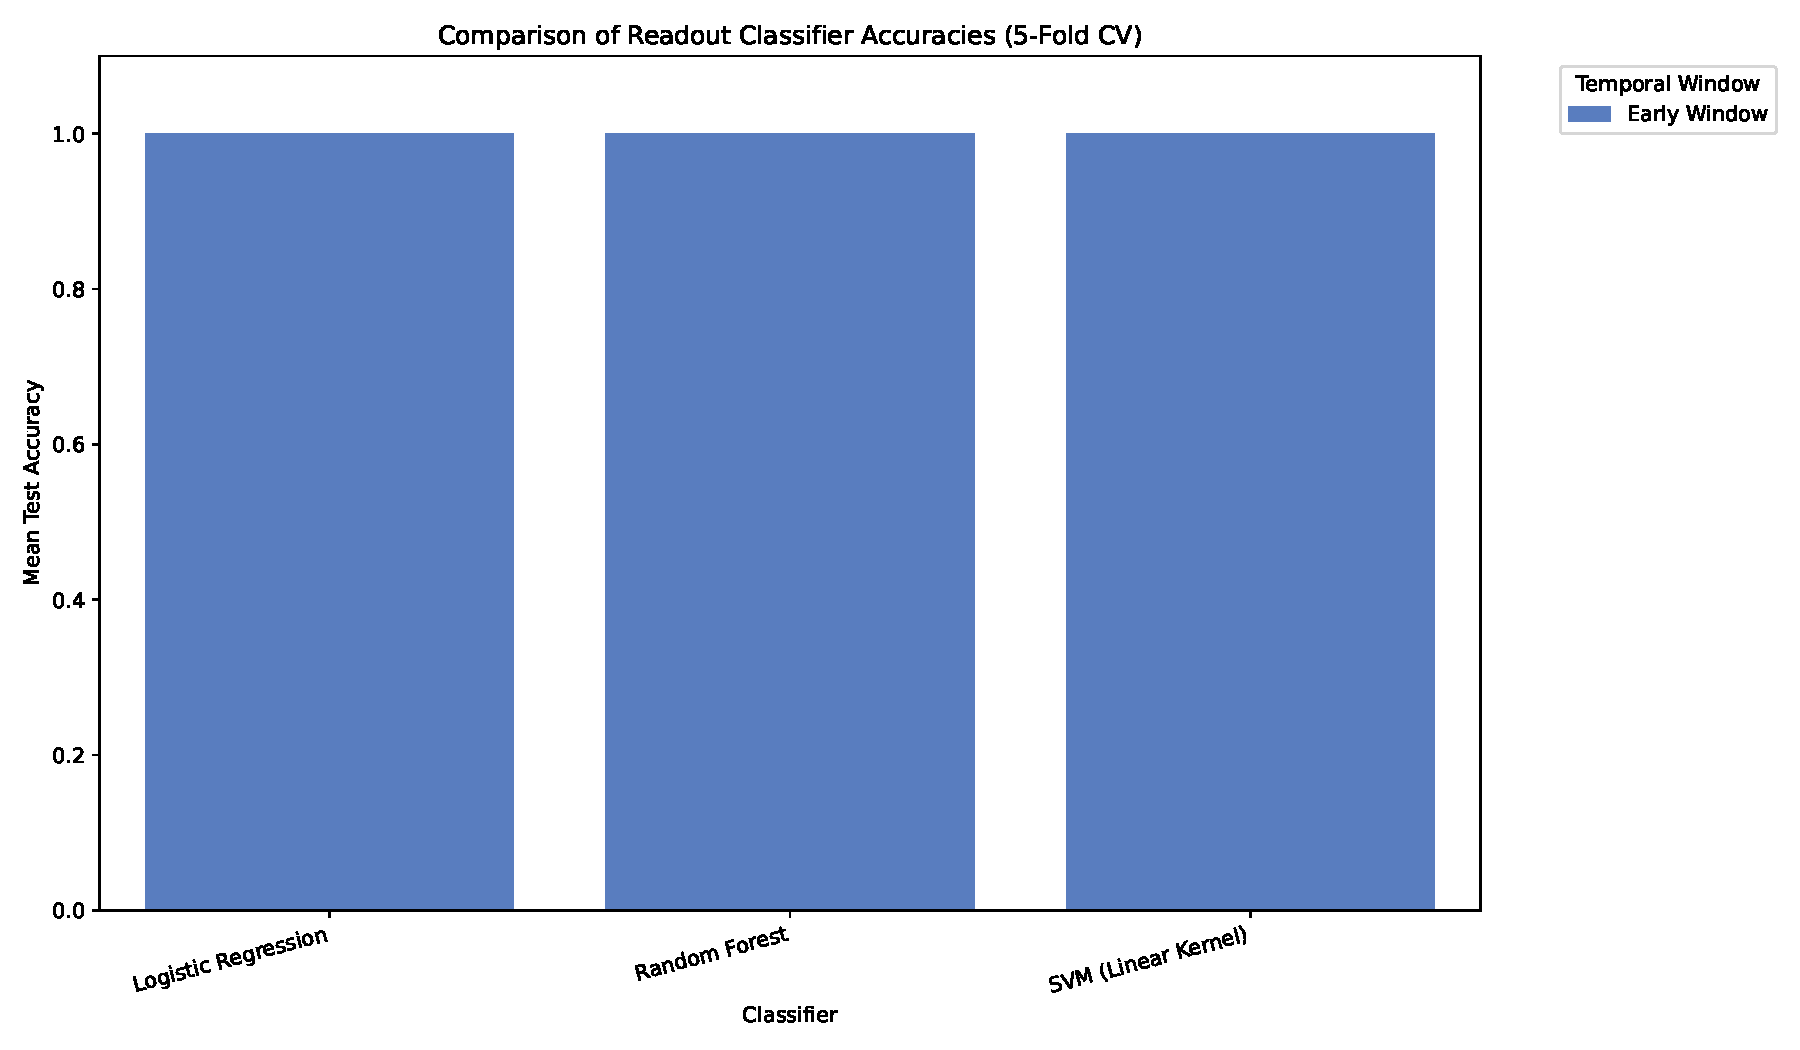
\includegraphics[width=0.8\textwidth]{pictures/chLSM/classifier_accuracy_comparison.pdf}
    \caption{Mean test accuracy (5-fold CV) for three readout classifiers on Early Window mean firing rates. All achieve perfect accuracy with zero variance. $\beta = 0.05$, $M_{\text{th}} = 0.5$.}
    \label{fig:m4_classifier_accuracy_comparison_actual}
\end{figure}

\begin{figure}[H]
    \centering
    \begin{subfigure}{0.48\textwidth}
        \centering
        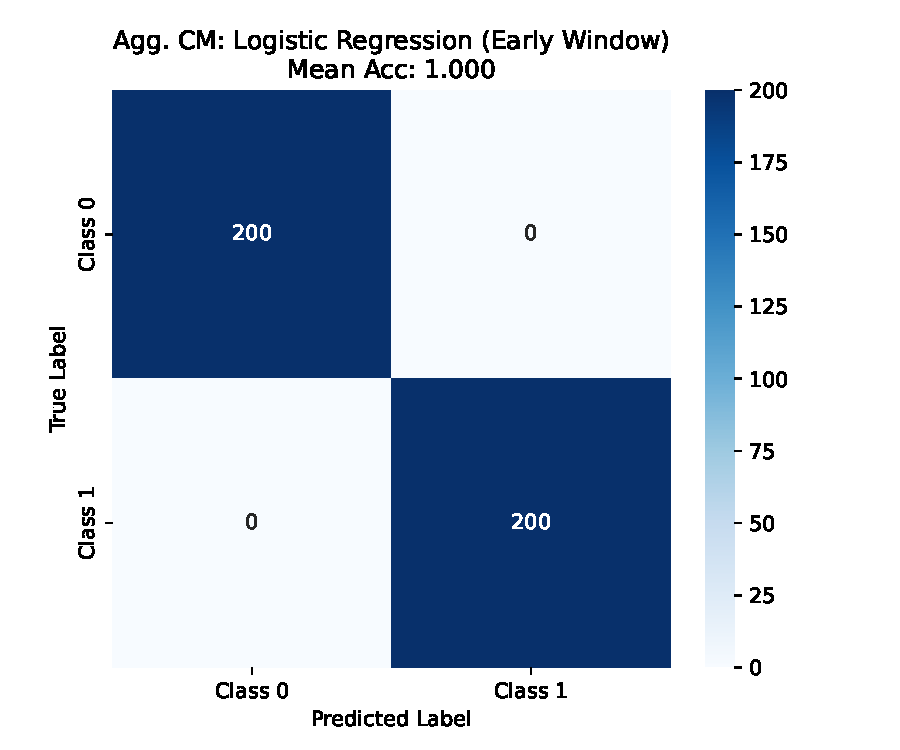
\includegraphics[width=\linewidth]{pictures/chLSM/cm_cv_logistic_regression_win_early_window.pdf}
        \caption{Logistic Regression (Acc: 1.000)}
        \label{fig:m4_cm_logreg_actual}
    \end{subfigure}
    \hfill
    \begin{subfigure}{0.48\textwidth}
        \centering
        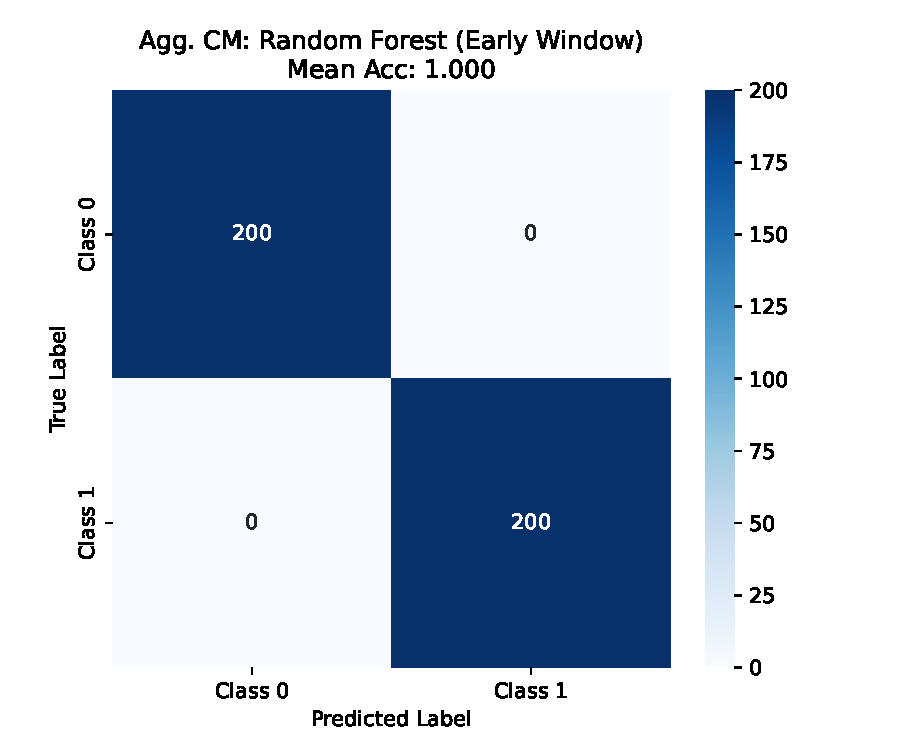
\includegraphics[width=\linewidth]{pictures/chLSM/cm_cv_random_forest_win_early_window.pdf}
        \caption{Random Forest (Acc: 1.000)}
        \label{fig:m4_cm_rf_actual}
    \end{subfigure}
    \vspace{1em}
    \begin{subfigure}{0.48\textwidth}
        \centering
        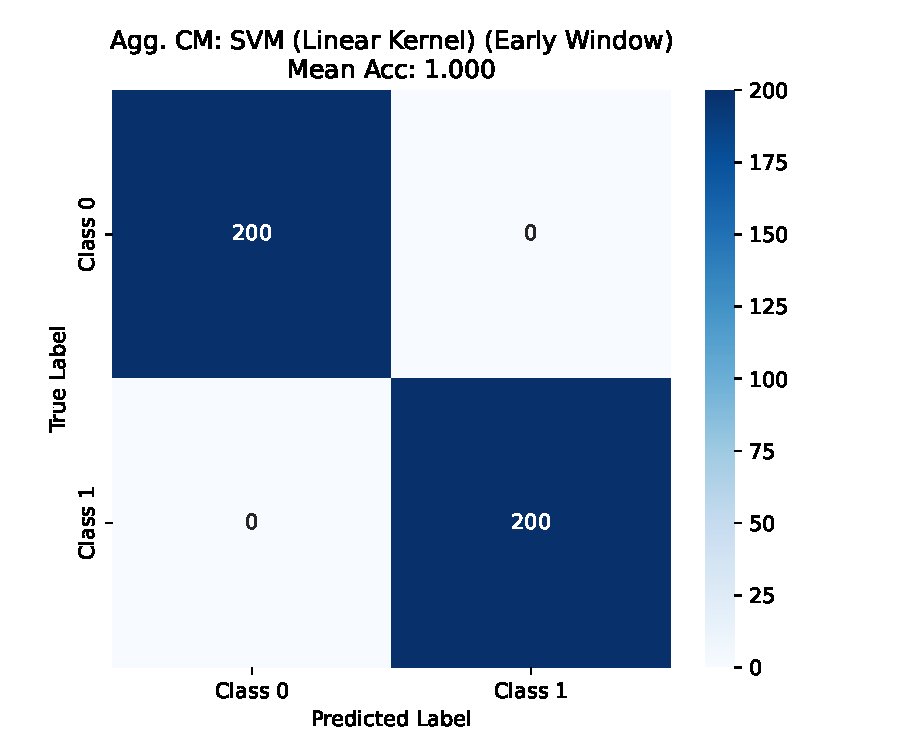
\includegraphics[width=\linewidth]{pictures/chLSM/cm_cv_svm_(linear_kernel)_win_early_window.pdf}
        \caption{SVM, Linear Kernel (Acc: 1.000)}
        \label{fig:m4_cm_svm_linear_actual}
    \end{subfigure}
    \caption{Aggregated confusion matrices (5-fold CV). All classifiers achieve perfect discrimination. $\beta = 0.05$, $M_{\text{th}} = 0.5$.}
    \label{fig:m4_confusion_matrices_all_actual}
\end{figure}

\subsection{Discussion and Significance}
\label{sec:module4_discussion}

\subsubsection{Confirmation of the Reservoir's Representational Purpose}

The uniform ceiling performance across linear and nonlinear classifiers confirms that the two stimulus classes are linearly separable in the 512-dimensional feature space. The nonlinear capacity of Random Forest was not required to achieve perfect separation. This is the expected outcome of a well-functioning reservoir: the fixed recurrent dynamics, threshold-based spiking, and high-dimensional projection collectively map two input signals that differ in a single scalar parameter into a representation where they occupy non-overlapping half-spaces demarcated by a hyperplane.

Mathematically, two classes $\mathcal{A}$ and $\mathcal{B}$ in $\mathbb{R}^n$ are linearly separable if there exists a weight vector $\mathbf{w} \in \mathbb{R}^n$ and a bias $b \in \mathbb{R}$ such that $\mathbf{w}^\top \mathbf{x}_a + b > 0$ for all $\mathbf{x}_a \in \mathcal{A}$ and $\mathbf{w}^\top \mathbf{x}_b + b \leq 0$ for all $\mathbf{x}_b \in \mathcal{B}$. The perfect accuracy of both linear classifiers confirms this condition is met. The reservoir has successfully performed the core function of reservoir computing: transforming a pattern classification problem into one solvable by a linear readout.

\subsubsection{Scope of the Controlled Result}

Three considerations define the scope of this result.

First, the task is deliberately simple: a binary discrimination between two constant-amplitude pulses with a $\sim$67\% amplitude difference and no additive noise, no inter-trial variability, and no temporal overlap between classes. The ceiling accuracy reflects the low intrinsic difficulty of this particular task as much as the quality of the reservoir transformation. This simplicity is intentional: it isolates the reservoir's representational transformation under maximally transparent conditions. An energy detector---summing the squared input amplitude---would also achieve perfect accuracy on this task. The reservoir's distinctive contribution becomes apparent on more complex tasks where the mapping from input to class is nonlinear and high-dimensional, as studied with real EEG in Chapter~\ref{chap:arspi_net}.

Second, the result establishes that the reservoir improves the \emph{representation geometry} for the chosen decoder---it does not establish that the reservoir creates new information about the class label. As the data processing inequality guarantees (Chapter~\ref{chap:background}, Section~\ref{sec:info_theory}), any processing of the input through a fixed transformation can only preserve or lose information about the latent class variable. When Chapter~\ref{chap:embeddings} reports that the Fisher Discriminant Ratio increases after the reservoir transformation, the correct interpretation is improved separability for linear readouts, not increased mutual information.

Third, linear separability under this controlled task does not guarantee separability under real EEG conditions, where class structure is weaker, noise is substantially greater, and inter-subject variability introduces systematic confounds. The demonstrated separability is a necessary but not sufficient condition for the utility of LSM-derived embeddings in the full ARSPI-Net architecture.

\subsubsection{What This Means for ARSPI-Net}

Within this scope, the result carries genuine engineering significance at several levels.

At the representation level, it demonstrates that the reservoir, at the validated operating point ($\beta = 0.05$, $M_{\text{th}} = 0.5$), produces well-structured embeddings whose discriminative content is concentrated in the early post-stimulus window and is accessible to simple linear readouts. The fact that a linear readout suffices means that the nonlinear transformation performed by the reservoir has already done the hard representational work: it has converted a one-dimensional amplitude difference into a pattern of differential firing rates across 512 neurons that can be read out by a hyperplane. The ``complexity'' of the classification problem, in a representation-theoretic sense, has been absorbed by the reservoir dynamics.

At the architectural level, this has a specific consequence for the graph model in Chapter~\ref{chap:arspi_net}. In a GNN, each node receives an initial feature vector, and the message-passing layers propagate information between neighbors. If the initial node features are already well-separated with respect to the classification target, the GNN can focus its learnable capacity on modeling \emph{inter-node relational structure}---how the patterns of activity across electrodes relate to the classification target---rather than spending capacity on disentangling poorly separated features within each node. This is the division of labor that the ARSPI-Net architecture is designed to exploit: the LSM handles temporal feature extraction per channel, and the GNN handles relational inference across channels. Module 4 provides the component-level evidence that the LSM side of this division is functioning as intended.

At the information-theoretic level, the result must be interpreted through the lens of the data processing inequality (DPI). The reservoir is a fixed transformation of the input; by DPI, the mutual information between the class label and the reservoir output cannot exceed the mutual information between the class label and the input. The reservoir's contribution is not to \emph{create} discriminative information but to \emph{reorganize} it into a form that is more accessible to a linear readout. This reorganization is achieved through the nonlinear dimensionality expansion: the 33-dimensional input is projected into a 512-dimensional space through the interplay of input weights, recurrent dynamics, and threshold-based spiking. The Fisher Discriminant Ratio analysis in Chapter~\ref{chap:embeddings} will quantify this reorganization more precisely by comparing the between-class to within-class scatter ratios before and after the reservoir transformation. The correct interpretation of any increase in FDR is improved representation geometry for linear decoders, not increased mutual information---a distinction that is critical for the intellectual integrity of the dissertation's claims.


%% ===================================================================
%% CHAPTER SYNTHESIS
%% ===================================================================
\section{Chapter Synthesis: Toward ARSPI-Net Integration}
\label{sec:chapter3_synthesis}

The systematic characterization conducted in this chapter establishes a set of controlled-design observations that inform, but do not by themselves validate, the later ARSPI-Net architecture. Critically, every observation in this chapter is traceable to a specific dynamical mechanism with a known mathematical description: the temporal integration window is governed by the LIF membrane time constant (Module~1), the state-space contraction is produced by the threshold-and-reset nonlinearity (Module~2), the temporal localization is consistent with the fading-memory kernel (Module~3), and the linear separability is consistent with the Koopman linearization principle (Module~4). This traceability is the foundational layer of ARSPI-Net's intrinsic interpretability: the reservoir's behavior is not a black box but an inspectable dynamical system whose operating regime is fully characterized by named, measurable parameters.

\subsection{Convergent Design Specifications}
\label{sec:design_specifications}

The experimental investigations across Modules~1--4 support the following provisional design conclusions:

\begin{enumerate}
    \item \textbf{Temporal control} (Module~1): The choice $\beta = 0.05$ balances persistence and responsiveness for the stimulus windows studied here, consistent with the low-pass filtering interpretation of the LIF kernel. The operating point is carried forward into subsequent chapters, where its adequacy on real EEG is empirically verified.

    \item \textbf{Response regime} (Module~2): The threshold $M_{\text{th}} = 0.5$ places the reservoir in a spike-generating regime whose population-level responses are substantially more stable across initializations than the subthreshold alternative. The spiking nonlinearity acts as a state-space contraction that regularizes the population code, making it a more defensible basis for downstream feature extraction.

    \item \textbf{Information localization} (Module~3): For the synthetic pulse family, discriminative information accessible via mean firing rates is concentrated in the early post-stimulus window (steps 20--50), with exponential decay consistent with the single-neuron fading-memory timescale. Chapter~\ref{chap:arspi_net} re-tests this temporal localization on real EEG, where the broadband spectral content and inter-trial variability of affective signals may alter the temporal profile.

    \item \textbf{Readout adequacy} (Module~4): Simple linear readouts suffice for the controlled task, confirming that the reservoir has achieved its intended representational purpose of projecting the input into a linearly separable space. The adequacy of linear readouts on the more complex real-EEG task is examined in Chapter~\ref{chap:arspi_net}.
\end{enumerate}

\subsection{Operating Point Specification}
\label{sec:validated_configuration}

These findings converge on the operating point specification summarized in Table~\ref{tab:ch3_config}. Chapter~\ref{chap:embeddings} refines several of these settings---reducing the reservoir size to 256 neurons (based on a saturation analysis), expanding the feature window to steps 10--70, and replacing mean firing rates with temporally resolved binned spike counts (BSC$_6$) reduced to 64 dimensions via PCA.

\begin{table}[htbp]
\centering
\small
\caption{Operating point specification from controlled characterization. Chapter~\ref{chap:embeddings} refines the reservoir size to 256, the feature window to steps 10--70, and the feature type to BSC$_6$ with PCA-64 reduction.}
\label{tab:ch3_config}
\renewcommand{\arraystretch}{1.2}
\begin{tabularx}{\textwidth}{|>{\raggedright\arraybackslash}p{3.5cm}|>{\centering\arraybackslash}p{2.5cm}|>{\raggedright\arraybackslash}X|}
\hline
\textbf{Parameter} & \textbf{Value} & \textbf{Rationale} \\
\hline
Membrane decay ($\beta$) & 0.05 & Balances persistence and responsiveness; $\tau_m \approx 20$ steps (Module~1) \\
\hline
Firing threshold ($M_{\text{th}}$) & 0.5 & Stable spiking regime with graded population encoding (Module~2) \\
\hline
Feature window & Steps 20--50 & Concentration of mean-rate discriminative content (Module~3) \\
\hline
Reservoir size & 512 neurons & Characterization configuration; saturates at 256 (Chapter~\ref{chap:embeddings}) \\
\hline
Feature type & Mean firing rates & Baseline representation; refined to BSC$_6$ in Chapter~\ref{chap:embeddings} \\
\hline
Readout & Linear classifier & Adequate for the controlled task; confirms linear separability (Module~4) \\
\hline
\end{tabularx}
\end{table}

The demonstrated linear separability of the reservoir features confirms that the reservoir performs a meaningful nonlinear transformation of representation geometry, consistent with Cover's theorem on pattern separability in high-dimensional nonlinear projections (Chapter~\ref{chap:background}, Section~\ref{sec:rc_theory}). The reservoir reorganizes the input into a geometric arrangement where the class boundary is linearly accessible---the specific contribution that motivates the BSC$_6$ temporal coding refinement in Chapter~\ref{chap:embeddings} and the graph-based spatial analysis in Chapter~\ref{chap:arspi_net}.

\subsection{Implications for the Dissertation}
\label{sec:ch3_implications}

The four modules jointly establish a coherent picture of the reservoir's behavior under controlled stimulation. The implications for the rest of the dissertation operate at three levels: architectural, methodological, and theoretical.

\subsubsection{Architectural Implications}

The central architectural lesson is a \emph{robustness hierarchy}: the subthreshold regime exhibited strong initialization sensitivity and ambiguous analog responses, whereas the spiking regime yielded substantially more stable and interpretable output through the regularizing effect of the threshold-and-reset nonlinearity. Spike-based operation is therefore the more defensible basis for constructing the node embeddings that the graph model in Chapter~\ref{chap:arspi_net} will consume. The linear separability demonstrated in Module~4 further implies that the GNN's role is to learn inter-electrode relational structure, not to compensate for poorly separated node features---a clean division of labor between the temporal (LSM) and spatial (GNN) components of the architecture.

\subsubsection{Methodological Implications}

The temporal localization finding has two downstream methodological consequences. For Chapter~\ref{chap:embeddings}, it motivates the search for richer coding schemes (such as binned spike counts) that can capture temporal structure beyond what mean rates provide. The chance-level late-window result in Module~3 is a positive constraint on the embedding design: features should be concentrated in the temporal region where the reservoir state is maximally driven, and any coding scheme that extends into later windows must use temporally resolved representations (not averages) to capture whatever residual structure may persist.

For Chapter~\ref{chap:arspi_net}, the temporal localization result establishes the hypothesis that the early post-stimulus window will remain the most informative region under real EEG conditions---a hypothesis that must be explicitly tested rather than assumed, because the nonstationarity, broadband spectral content, and inter-trial variability of real EEG could substantially alter the temporal profile of discriminative information in the reservoir state.

\subsubsection{Theoretical Implications}

Chapter~\ref{chap:dynamics} exploits the same reservoir trajectories from a complementary perspective. Rather than extracting discriminative features for classification, it characterizes the driven reservoir as a nonlinear dynamical system and asks whether state-space descriptors---Lyapunov exponents, Lempel-Ziv complexity, permutation entropy, and relaxation times---can serve as interpretable biomarkers of the input process. The controlled characterization of the reservoir's operating regime in the present chapter is a prerequisite for that analysis in two specific ways. First, the dynamical metrics in Chapter~\ref{chap:dynamics} are meaningful only if the reservoir satisfies the Echo State Property under the relevant input class, which requires the reservoir to be in a stable, well-characterized operating regime rather than in an uncontrolled or chaotic state. The spiking regime validated in Module~2 is more likely to satisfy ESP than the subthreshold regime, because the threshold-and-reset contraction provides a mechanism for state-space convergence that the linear subthreshold dynamics lack. Second, the temporal localization result informs the choice of analysis windows for the dynamical metrics: the sparse coding efficiency and trajectory complexity measures in Chapter~\ref{chap:dynamics} should be computed over the same post-stimulus window where the reservoir state is maximally driven and most informative.

Chapter~\ref{chap:synthesis} then closes the loop by asking whether the dynamical descriptors from Chapter~\ref{chap:dynamics} and the graph-topological descriptors from Chapter~\ref{chap:arspi_net} are statistically coupled---that is, whether electrodes with rich dynamical signatures also occupy distinctive positions in the functional graph. The present chapter's demonstration that the reservoir produces consistent, interpretable responses to controlled input provides the empirical foundation for believing that such coupling analysis is meaningful rather than arbitrary.

\subsection{Forward-Looking Design Principles}

The controlled characterization establishes five design principles that propagate through the remaining chapters:
\begin{itemize}
    \item Spike-based operation produces more stable and reproducible population codes than subthreshold dynamics, making it the appropriate basis for the embedding pipeline (Chapter~\ref{chap:embeddings}) and for the dynamical trajectory analysis (Chapter~\ref{chap:dynamics}).
    \item Temporal windowing is a first-class design variable. The concentration of discriminative information in the early post-stimulus window motivates both the BSC$_6$ temporal binning strategy (Chapter~\ref{chap:embeddings}) and the analysis windows for dynamical metrics (Chapter~\ref{chap:dynamics}).
    \item Embedding quality determines the ceiling for downstream analysis. The linear separability achieved by the reservoir's nonlinear transformation motivates the representation engineering of Chapter~\ref{chap:embeddings}, where the coding scheme is refined to capture temporal structure that mean rates cannot access.
    \item \textbf{Interpretability is preserved at every stage.} Because the reservoir weights are fixed and the operating regime is fully characterized, every downstream output---from spike rasters to temporal codes to dynamical descriptors---can be traced back to the input signal through the known dynamical equations. This traceability is not a post-hoc property; it is a design consequence of using a fixed, characterized nonlinear transformation rather than a learned one.
    \item The operating point validated here on synthetic stimuli is carried forward to real EEG processing, where its adequacy is empirically verified on the SHAPE dataset (Chapter~\ref{chap:arspi_net}).
\end{itemize}

This chapter establishes the first stage of the ARSPI-Net architecture: a controlled, characterized reservoir operating point that produces stable, interpretable spike-based representations of its driving input. Every parameter selection is justified by a named dynamical mechanism, and the reservoir's behavior under each regime is documented with quantitative precision---establishing the foundation for the intrinsic interpretability that distinguishes ARSPI-Net from black-box alternatives. This fixed-weight, fully characterized approach differs fundamentally from the STDP-based learning used in NeuCube \cite{kasabov_neucube_2014}, where the reservoir weights adapt during training and the resulting dynamics are a product of both the input and the learning rule. In ARSPI-Net, the reservoir dynamics are determined solely by the input signal and the known parameters ($\beta$, $\theta$, spectral radius)---a design choice that sacrifices adaptability for complete inspectability. Chapter~\ref{chap:embeddings} develops the representation engineering that converts these spike responses into compact, discriminative embeddings while preserving the temporal traceability established here. Together, they define the per-channel temporal encoding that feeds the multichannel spatial analysis in Chapters~\ref{chap:arspi_net}--\ref{chap:synthesis}.